%*************************************************************************
% A Classic Thesis Style
% An Homage to The Elements of Typographic Style
%
% Copyright (C) 2017 André Miede and Ivo Pletikosić
%
% If you like the style then I would appreciate a postcard. My address
% can be found in the file ClassicThesis.pdf. A collection of the
% postcards I received so far is available online at
% http://postcards.miede.de
%
% License:
% This program is free software; you can redistribute it and/or modify
% it under the terms of the GNU General Public License as published by
% the Free Software Foundation; either version 2 of the License, or
% (at your option) any later version.
%
% This program is distributed in the hope that it will be useful,
% but WITHOUT ANY WARRANTY; without even the implied warranty of
% MERCHANTABILITY or FITNESS FOR A PARTICULAR PURPOSE.  See the
% GNU General Public License for more details.
%
% You should have received a copy of the GNU General Public License
% along with this program; see the file COPYING.  If not, write to
% the Free Software Foundation, Inc., 59 Temple Place - Suite 330,
% Boston, MA 02111-1307, USA.
%
% PLEASE SEE ALSO THE AUTHORS' NOTE REGARDING THIS LICENSE
% IN THE DOCUMENTATION (ClassicThesis.pdf --> Chapter 1 / Chapter01.tex)
%*************************************************************************
\RequirePackage{silence} % :-\
    \WarningFilter{scrreprt}{Usage of package `titlesec'}
    %\WarningFilter{scrreprt}{Activating an ugly workaround}
    \WarningFilter{titlesec}{Non standard sectioning command detected}
\documentclass[ openright,titlepage,numbers=noenddot,headinclude,%twoside, %1headlines,% letterpaper a4paper
                footinclude=true,cleardoublepage=empty,
                BCOR=5mm,paper=a4,fontsize=11pt,%11pt,a4paper,%
                ngerman,american,%lockflag%
                ]{scrreprt}

%*************************************************************************
% Note: Make all your adjustments in here
%*************************************************************************
% ****************************************************************************************************
% hdathesis-config.tex 
% Use it at the beginning of your thesis.tex, or as a LaTeX Preamble 
% in your thesis.{tex,lyx} with % ****************************************************************************************************
% hdathesis-config.tex 
% Use it at the beginning of your thesis.tex, or as a LaTeX Preamble 
% in your thesis.{tex,lyx} with % ****************************************************************************************************
% hdathesis-config.tex 
% Use it at the beginning of your thesis.tex, or as a LaTeX Preamble 
% in your thesis.{tex,lyx} with \input{hdathesis-config}
% ****************************************************************************************************

% ****************************************************************************************************
% 1. Personal data and user ad-hoc commands
% ****************************************************************************************************
%\newcommand{\myTitle}{Datenschutz - Allgemeinwohl gegen Privacy \\ Wie viel Überwachung darf?\xspace}
\newcommand{\myTitle}{Improve Code Quality of Legacy Code\xspace}
\newcommand{\mySubtitle}{Am Beispiel von Natural C/C++ Code\xspace}
\newcommand{\myDegree}{Bachelor of Science (B.Sc.)\xspace} 
%\newcommand{\myDegree}{Bachelor of Arts (B.A.)\xspace}
%\newcommand{\myDegree}{Master of Science (M.Sc.)\xspace}
%\newcommand{\myDegree}{Master of Arts (M.A.)\xspace}
\newcommand{\myName}{Sandra Gräf\xspace}
\newcommand{\myId}{1111826\xspace}
\newcommand{\myMail}{sandra.graef@stud.h-da.de\xspace}
\newcommand{\myProf}{Prof. Dr. Oliver Weissmann\xspace}
\newcommand{\myOtherProf}{Prof. Dr. Ralf Hahn???????\xspace}
\newcommand{\myFaculty}{Fachbereich Informatik\xspace}
\newcommand{\myUni}{Hochschule Darmstadt\xspace}
\newcommand{\myLocation}{Darmstadt\xspace}
\newcommand{\myTime}{04. März 2025\xspace}
\newcommand{\myVersion}{version 1\xspace}

% ****************************************************************************************************
% 2. Is it a master thesis?
% ****************************************************************************************************
%\PassOptionsToPackage{master}{hdathesis} % uncomment if this is a master thesis 

% ****************************************************************************************************
% 3. Does the thesis have a lock flag?
% ****************************************************************************************************
%\PassOptionsToPackage{lockflag}{hdathesis} % uncomment if this thesis has a lock flag 

% ****************************************************************************************************
% 4. Loading some handy packages
% ****************************************************************************************************
% ****************************************************************************************************
% Packages with options that might require adjustments
% ****************************************************************************************************

%\PassOptionsToPackage{ngerman,american}{babel}   % change this to your language(s)
% Spanish languages need extra options in order to work with this template
%\PassOptionsToPackage{spanish,es-lcroman}{babel}
\usepackage{babel}


% ****************************************************************************************************

% ****************************************************************************************************
% 1. Personal data and user ad-hoc commands
% ****************************************************************************************************
%\newcommand{\myTitle}{Datenschutz - Allgemeinwohl gegen Privacy \\ Wie viel Überwachung darf?\xspace}
\newcommand{\myTitle}{Improve Code Quality of Legacy Code\xspace}
\newcommand{\mySubtitle}{Am Beispiel von Natural C/C++ Code\xspace}
\newcommand{\myDegree}{Bachelor of Science (B.Sc.)\xspace} 
%\newcommand{\myDegree}{Bachelor of Arts (B.A.)\xspace}
%\newcommand{\myDegree}{Master of Science (M.Sc.)\xspace}
%\newcommand{\myDegree}{Master of Arts (M.A.)\xspace}
\newcommand{\myName}{Sandra Gräf\xspace}
\newcommand{\myId}{1111826\xspace}
\newcommand{\myMail}{sandra.graef@stud.h-da.de\xspace}
\newcommand{\myProf}{Prof. Dr. Oliver Weissmann\xspace}
\newcommand{\myOtherProf}{Prof. Dr. Ralf Hahn???????\xspace}
\newcommand{\myFaculty}{Fachbereich Informatik\xspace}
\newcommand{\myUni}{Hochschule Darmstadt\xspace}
\newcommand{\myLocation}{Darmstadt\xspace}
\newcommand{\myTime}{04. März 2025\xspace}
\newcommand{\myVersion}{version 1\xspace}

% ****************************************************************************************************
% 2. Is it a master thesis?
% ****************************************************************************************************
%\PassOptionsToPackage{master}{hdathesis} % uncomment if this is a master thesis 

% ****************************************************************************************************
% 3. Does the thesis have a lock flag?
% ****************************************************************************************************
%\PassOptionsToPackage{lockflag}{hdathesis} % uncomment if this thesis has a lock flag 

% ****************************************************************************************************
% 4. Loading some handy packages
% ****************************************************************************************************
% ****************************************************************************************************
% Packages with options that might require adjustments
% ****************************************************************************************************

%\PassOptionsToPackage{ngerman,american}{babel}   % change this to your language(s)
% Spanish languages need extra options in order to work with this template
%\PassOptionsToPackage{spanish,es-lcroman}{babel}
\usepackage{babel}


% ****************************************************************************************************

% ****************************************************************************************************
% 1. Personal data and user ad-hoc commands
% ****************************************************************************************************
%\newcommand{\myTitle}{Datenschutz - Allgemeinwohl gegen Privacy \\ Wie viel Überwachung darf?\xspace}
\newcommand{\myTitle}{Improve Code Quality of Legacy Code\xspace}
\newcommand{\mySubtitle}{Am Beispiel von Natural C/C++ Code\xspace}
\newcommand{\myDegree}{Bachelor of Science (B.Sc.)\xspace} 
%\newcommand{\myDegree}{Bachelor of Arts (B.A.)\xspace}
%\newcommand{\myDegree}{Master of Science (M.Sc.)\xspace}
%\newcommand{\myDegree}{Master of Arts (M.A.)\xspace}
\newcommand{\myName}{Sandra Gräf\xspace}
\newcommand{\myId}{1111826\xspace}
\newcommand{\myMail}{sandra.graef@stud.h-da.de\xspace}
\newcommand{\myProf}{Prof. Dr. Oliver Weissmann\xspace}
\newcommand{\myOtherProf}{Prof. Dr. Ralf Hahn???????\xspace}
\newcommand{\myFaculty}{Fachbereich Informatik\xspace}
\newcommand{\myUni}{Hochschule Darmstadt\xspace}
\newcommand{\myLocation}{Darmstadt\xspace}
\newcommand{\myTime}{04. März 2025\xspace}
\newcommand{\myVersion}{version 1\xspace}

% ****************************************************************************************************
% 2. Is it a master thesis?
% ****************************************************************************************************
%\PassOptionsToPackage{master}{hdathesis} % uncomment if this is a master thesis 

% ****************************************************************************************************
% 3. Does the thesis have a lock flag?
% ****************************************************************************************************
%\PassOptionsToPackage{lockflag}{hdathesis} % uncomment if this thesis has a lock flag 

% ****************************************************************************************************
% 4. Loading some handy packages
% ****************************************************************************************************
% ****************************************************************************************************
% Packages with options that might require adjustments
% ****************************************************************************************************

%\PassOptionsToPackage{ngerman,american}{babel}   % change this to your language(s)
% Spanish languages need extra options in order to work with this template
%\PassOptionsToPackage{spanish,es-lcroman}{babel}
\usepackage{babel}


% ****************************************************************************************************
% classicthesis-config.tex
% formerly known as loadpackages.sty, classicthesis-ldpkg.sty, and classicthesis-preamble.sty
% Use it at the beginning of your ClassicThesis.tex, or as a LaTeX Preamble
% in your ClassicThesis.{tex,lyx} with % ****************************************************************************************************
% classicthesis-config.tex
% formerly known as loadpackages.sty, classicthesis-ldpkg.sty, and classicthesis-preamble.sty
% Use it at the beginning of your ClassicThesis.tex, or as a LaTeX Preamble
% in your ClassicThesis.{tex,lyx} with % ****************************************************************************************************
% classicthesis-config.tex
% formerly known as loadpackages.sty, classicthesis-ldpkg.sty, and classicthesis-preamble.sty
% Use it at the beginning of your ClassicThesis.tex, or as a LaTeX Preamble
% in your ClassicThesis.{tex,lyx} with \input{classicthesis-config}
% ****************************************************************************************************
% If you like the classicthesis, then I would appreciate a postcard.
% My address can be found in the file ClassicThesis.pdf. A collection
% of the postcards I received so far is available online at
% http://postcards.miede.de
% ****************************************************************************************************


% ****************************************************************************************************
% 0. Set the encoding of your files. UTF-8 is the only sensible encoding nowadays. If you can't read
% äöüßáéçèê∂åëæƒÏ€ then change the encoding setting in your editor, not the line below. If your editor
% does not support utf8 use another editor!
% ****************************************************************************************************
\PassOptionsToPackage{utf8}{inputenc}
  \usepackage{inputenc}

% ****************************************************************************************************
% 1. Configure classicthesis for your needs here, e.g., remove "drafting" below
% in order to deactivate the time-stamp on the pages
% (see ClassicThesis.pdf for more information):
% ****************************************************************************************************
\PassOptionsToPackage{
  drafting=false,   % print version information on the bottom of the pages
  tocaligned=false, % the left column of the toc will be aligned (no indentation)
  dottedtoc=true,   % page numbers in ToC flushed right
  parts=true,       % use part division
  eulerchapternumbers=true, % use AMS Euler for chapter font (otherwise Palatino)
  linedheaders=false,       % chaper headers will have line above and beneath
  floatperchapter=true,     % numbering per chapter for all floats (i.e., Figure 1.1)
  listings=true,    % load listings package and setup LoL
  subfig=true,      % setup for preloaded subfig package
  eulermath=false,  % use awesome Euler fonts for mathematical formulae (only with pdfLaTeX)
  beramono=true,    % toggle a nice monospaced font (w/ bold)
  minionpro=false   % setup for minion pro font; use minion pro small caps as well (only with pdfLaTeX)
}{classicthesis}


% ****************************************************************************************************
% 2. Personal data and user ad-hoc commands
% ****************************************************************************************************
%\newcommand{\myTitle}{A Classic Thesis Style\xspace}
%\newcommand{\mySubtitle}{An Homage to The Elements of Typographic Style\xspace}
%\newcommand{\myDegree}{Doktor-Ingenieur (Dr.-Ing.)\xspace}
%\newcommand{\myName}{André Miede\xspace}
%\newcommand{\myProf}{Put name here\xspace}
%\newcommand{\myOtherProf}{Put name here\xspace}
%\newcommand{\mySupervisor}{Put name here\xspace}
%\newcommand{\myFaculty}{Put data here\xspace}
%\newcommand{\myDepartment}{Put data here\xspace}
%\newcommand{\myUni}{Put data here\xspace}
%\newcommand{\myLocation}{Saarbrücken\xspace}
%\newcommand{\myTime}{October 2017\xspace}
%\newcommand{\myVersion}{version 4.4}

% ********************************************************************
% Setup, finetuning, and useful commands
% ********************************************************************
\newcounter{dummy} % necessary for correct hyperlinks (to index, bib, etc.)
\newlength{\abcd} % for ab..z string length calculation
\providecommand{\mLyX}{L\kern-.1667em\lower.25em\hbox{Y}\kern-.125emX\@}
\newcommand{\ie}{i.\,e.}
\newcommand{\Ie}{I.\,e.}
\newcommand{\eg}{e.\,g.}
\newcommand{\Eg}{E.\,g.}
% ****************************************************************************************************


% ****************************************************************************************************
% 3. Loading some handy packages
% ****************************************************************************************************
% ********************************************************************
% Packages with options that might require adjustments
% ********************************************************************
%\PassOptionsToPackage{ngerman,american}{babel}   % change this to your language(s), main language last
% Spanish languages need extra options in order to work with this template
%\PassOptionsToPackage{spanish,es-lcroman}{babel}
\usepackage{babel}

\usepackage{csquotes}
%\usepackage{hyperref}
%\usepackage[figure]{hypcap}

\PassOptionsToPackage{%
  %backend=biber,bibencoding=utf8, %instead of bibtex
  backend=bibtex8,bibencoding=ascii,%
  language=auto,%
  %style=numeric-comp,%
  style=alphabetic,%
  %style=authoryear-comp, % Author 1999, 2010
  %bibstyle=authoryear,dashed=false, % dashed: substitute rep. author with ---
  sorting=nyt, % name, year, title
  maxbibnames=10, % default: 3, et al.
  %backref=true,%
  natbib=true % natbib compatibility mode (\citep and \citet still work)
}{biblatex}
  \usepackage{biblatex}

\PassOptionsToPackage{fleqn}{amsmath}       % math environments and more by the AMS
  \usepackage{amsmath}

\PassOptionsToPackage{doublespacing}{hdathesis}  % options: abbrev exam big wiwi english master
  \usepackage{hdathesis}

% ********************************************************************
% General useful packages
% ********************************************************************
\PassOptionsToPackage{T1}{fontenc} % T2A for cyrillics
  \usepackage{fontenc}
\usepackage{textcomp} % fix warning with missing font shapes
\usepackage{scrhack} % fix warnings when using KOMA with listings package
\usepackage{xspace} % to get the spacing after macros right
\usepackage{mparhack} % get marginpar right
%\usepackage{fixltx2e} % fixes some LaTeX stuff --> since 2015 in the LaTeX kernel (see below)
% \usepackage[latest]{latexrelease} % emulate newer kernel version if older is detected
\PassOptionsToPackage{printonlyused,smaller}{acronym}
  \usepackage{acronym} % nice macros for handling all acronyms in the thesis
  %\renewcommand{\bflabel}[1]{{#1}\hfill} % fix the list of acronyms --> no longer working
  %\renewcommand*{\acsfont}[1]{\textsc{#1}}
  %\renewcommand*{\aclabelfont}[1]{\acsfont{#1}}
  %\def\bflabel#1{{#1\hfill}}
  \def\bflabel#1{{\acsfont{#1}\hfill}}
  \def\aclabelfont#1{\acsfont{#1}}
% ****************************************************************************************************
%\usepackage{pgfplots} % External TikZ/PGF support (thanks to Andreas Nautsch)
%\usetikzlibrary{external}
%\tikzexternalize[mode=list and make, prefix=ext-tikz/]
% ****************************************************************************************************


% ****************************************************************************************************
% 4. Setup floats: tables, (sub)figures, and captions
% ****************************************************************************************************
\usepackage{tabularx} % better tables
  \setlength{\extrarowheight}{3pt} % increase table row height
\newcommand{\tableheadline}[1]{\multicolumn{1}{c}{\spacedlowsmallcaps{#1}}}
\newcommand{\myfloatalign}{\centering} % to be used with each float for alignment
\usepackage{caption}
% Thanks to cgnieder and Claus Lahiri
% http://tex.stackexchange.com/questions/69349/spacedlowsmallcaps-in-caption-label
% [REMOVED DUE TO OTHER PROBLEMS, SEE ISSUE #82]
%\DeclareCaptionLabelFormat{smallcaps}{\bothIfFirst{#1}{~}\MakeTextLowercase{\textsc{#2}}}
%\captionsetup{font=small,labelformat=smallcaps} % format=hang,
\captionsetup{font=small} % format=hang,
\usepackage{subfig}
% ****************************************************************************************************


% ****************************************************************************************************
% 5. Setup code listings
% ****************************************************************************************************
\usepackage{listings}
%\lstset{emph={trueIndex,root},emphstyle=\color{BlueViolet}}%\underbar} % for special keywords
\lstset{language=[LaTeX]Tex,%C++,
  morekeywords={PassOptionsToPackage,selectlanguage},
  keywordstyle=\color{RoyalBlue},%\bfseries,
  basicstyle=\small\ttfamily,
  %identifierstyle=\color{NavyBlue},
  commentstyle=\color{Green}\ttfamily,
  stringstyle=\rmfamily,
  numbers=none,%left,%
  numberstyle=\scriptsize,%\tiny
  stepnumber=5,
  numbersep=8pt,
  showstringspaces=false,
  breaklines=true,
  %frameround=ftff,
  %frame=single,
  belowcaptionskip=.75\baselineskip
  %frame=L
}
% ****************************************************************************************************


% ****************************************************************************************************
% 6. PDFLaTeX, hyperreferences, and citation backreferences
% ****************************************************************************************************
% ********************************************************************
% Using PDFLaTeX
% ********************************************************************
\PassOptionsToPackage{hyperfootnotes=false,pdfpagelabels}{hyperref}
\usepackage{hyperref}  % backref linktocpage pagebackref
%\ifpdf
%\pdfcompresslevel=9
%\pdfadjustspacing=1
%\fi
%\PassOptionsToPackage{pdftex}{graphicx} %%%IVO: driver will be chosen automatically
\usepackage{graphicx}
\usepackage{subcaption}


% ********************************************************************
% Hyperreferences
% ********************************************************************
\hypersetup{%
  %draft, % hyperref's draft mode, for printing see below
  colorlinks=true, linktocpage=true, pdfstartpage=1, pdfstartview=FitV,%
  % uncomment the following line if you want to have black links (e.g., for printing)
  %colorlinks=false, linktocpage=false, pdfstartpage=3, pdfstartview=FitV, pdfborder={0 0 0},%
  breaklinks=true, pdfpagemode=UseNone, pageanchor=true, pdfpagemode=UseOutlines,%
  plainpages=false, bookmarksnumbered, bookmarksopen=true, bookmarksopenlevel=1,%
  hypertexnames=true, pdfhighlight=/O,%nesting=true,%frenchlinks,%
  urlcolor=webbrown, linkcolor=RoyalBlue, citecolor=webgreen, %pagecolor=RoyalBlue,%
  %urlcolor=Black, linkcolor=Black, citecolor=Black, %pagecolor=Black,%
  pdftitle={\myTitle},%
  pdfauthor={\textcopyright\ \myName, \myUni, \myFaculty},%
  pdfsubject={},%
  pdfkeywords={},%
  pdfcreator={pdfLaTeX},%
  pdfproducer={LaTeX with hyperref and classicthesis}%
}

% ********************************************************************
% Setup autoreferences
% ********************************************************************
% There are some issues regarding autorefnames
% http://www.ureader.de/msg/136221647.aspx
% http://www.tex.ac.uk/cgi-bin/texfaq2html?label=latexwords
% you have to redefine the makros for the
% language you use, e.g., american, ngerman
% (as chosen when loading babel/AtBeginDocument)
% ********************************************************************
\makeatletter
\@ifpackageloaded{babel}%
  {%
    \addto\extrasamerican{%
      \renewcommand*{\figureautorefname}{Figure}%
      \renewcommand*{\tableautorefname}{Table}%
      \renewcommand*{\partautorefname}{Part}%
      \renewcommand*{\chapterautorefname}{Chapter}%
      \renewcommand*{\sectionautorefname}{Section}%
      \renewcommand*{\subsectionautorefname}{Section}%
      \renewcommand*{\subsubsectionautorefname}{Section}%
    }%
    \addto\extrasngerman{%
      \renewcommand*{\paragraphautorefname}{Absatz}%
      \renewcommand*{\subparagraphautorefname}{Unterabsatz}%
      \renewcommand*{\footnoteautorefname}{Fu\"snote}%
      \renewcommand*{\FancyVerbLineautorefname}{Zeile}%
      \renewcommand*{\theoremautorefname}{Theorem}%
      \renewcommand*{\appendixautorefname}{Anhang}%
      \renewcommand*{\equationautorefname}{Gleichung}%
      \renewcommand*{\itemautorefname}{Punkt}%
    }%
      % Fix to getting autorefs for subfigures right (thanks to Belinda Vogt for changing the definition)
      \providecommand{\subfigureautorefname}{\figureautorefname}%
    }{\relax}
\makeatother


% ****************************************************************************************************
% 7. Last calls before the bar closes
% ****************************************************************************************************
% ********************************************************************
% Development Stuff
% ********************************************************************
\listfiles
%\PassOptionsToPackage{l2tabu,orthodox,abort}{nag}
%  \usepackage{nag}
%\PassOptionsToPackage{warning, all}{onlyamsmath}
%  \usepackage{onlyamsmath}

% ********************************************************************
% Last, but not least...
% ********************************************************************
\usepackage{classicthesis}
% ****************************************************************************************************


% ****************************************************************************************************
% 8. Further adjustments (experimental)
% ****************************************************************************************************
% ********************************************************************
% Changing the text area
% ********************************************************************
%\areaset[current]{312pt}{761pt} % 686 (factor 2.2) + 33 head + 42 head \the\footskip
%\setlength{\marginparwidth}{7em}%
%\setlength{\marginparsep}{2em}%

% ********************************************************************
% Using different fonts
% ********************************************************************
%\usepackage[oldstylenums]{kpfonts} % oldstyle notextcomp
%\usepackage[osf]{libertine}
%\usepackage[light,condensed,math]{iwona}
%\renewcommand{\sfdefault}{iwona}
%\usepackage{lmodern} % <-- no osf support :-(
%\usepackage{cfr-lm} %
%\usepackage[urw-garamond]{mathdesign} <-- no osf support :-(
%\usepackage[default,osfigures]{opensans} % scale=0.95
%\usepackage[sfdefault]{FiraSans}
% ********************************************************************
% \usepackage[largesc,osf]{newpxtext}
% Used to fix these:
% https://bitbucket.org/amiede/classicthesis/issues/139/italics-in-pallatino-capitals-chapter
% https://bitbucket.org/amiede/classicthesis/issues/45/problema-testatine-su-classicthesis-style
% ********************************************************************
%\linespread{1.05} % a bit more for Palatino
% ****************************************************************************************************

% ****************************************************************************************************
% If you like the classicthesis, then I would appreciate a postcard.
% My address can be found in the file ClassicThesis.pdf. A collection
% of the postcards I received so far is available online at
% http://postcards.miede.de
% ****************************************************************************************************


% ****************************************************************************************************
% 0. Set the encoding of your files. UTF-8 is the only sensible encoding nowadays. If you can't read
% äöüßáéçèê∂åëæƒÏ€ then change the encoding setting in your editor, not the line below. If your editor
% does not support utf8 use another editor!
% ****************************************************************************************************
\PassOptionsToPackage{utf8}{inputenc}
  \usepackage{inputenc}

% ****************************************************************************************************
% 1. Configure classicthesis for your needs here, e.g., remove "drafting" below
% in order to deactivate the time-stamp on the pages
% (see ClassicThesis.pdf for more information):
% ****************************************************************************************************
\PassOptionsToPackage{
  drafting=false,   % print version information on the bottom of the pages
  tocaligned=false, % the left column of the toc will be aligned (no indentation)
  dottedtoc=true,   % page numbers in ToC flushed right
  parts=true,       % use part division
  eulerchapternumbers=true, % use AMS Euler for chapter font (otherwise Palatino)
  linedheaders=false,       % chaper headers will have line above and beneath
  floatperchapter=true,     % numbering per chapter for all floats (i.e., Figure 1.1)
  listings=true,    % load listings package and setup LoL
  subfig=true,      % setup for preloaded subfig package
  eulermath=false,  % use awesome Euler fonts for mathematical formulae (only with pdfLaTeX)
  beramono=true,    % toggle a nice monospaced font (w/ bold)
  minionpro=false   % setup for minion pro font; use minion pro small caps as well (only with pdfLaTeX)
}{classicthesis}


% ****************************************************************************************************
% 2. Personal data and user ad-hoc commands
% ****************************************************************************************************
%\newcommand{\myTitle}{A Classic Thesis Style\xspace}
%\newcommand{\mySubtitle}{An Homage to The Elements of Typographic Style\xspace}
%\newcommand{\myDegree}{Doktor-Ingenieur (Dr.-Ing.)\xspace}
%\newcommand{\myName}{André Miede\xspace}
%\newcommand{\myProf}{Put name here\xspace}
%\newcommand{\myOtherProf}{Put name here\xspace}
%\newcommand{\mySupervisor}{Put name here\xspace}
%\newcommand{\myFaculty}{Put data here\xspace}
%\newcommand{\myDepartment}{Put data here\xspace}
%\newcommand{\myUni}{Put data here\xspace}
%\newcommand{\myLocation}{Saarbrücken\xspace}
%\newcommand{\myTime}{October 2017\xspace}
%\newcommand{\myVersion}{version 4.4}

% ********************************************************************
% Setup, finetuning, and useful commands
% ********************************************************************
\newcounter{dummy} % necessary for correct hyperlinks (to index, bib, etc.)
\newlength{\abcd} % for ab..z string length calculation
\providecommand{\mLyX}{L\kern-.1667em\lower.25em\hbox{Y}\kern-.125emX\@}
\newcommand{\ie}{i.\,e.}
\newcommand{\Ie}{I.\,e.}
\newcommand{\eg}{e.\,g.}
\newcommand{\Eg}{E.\,g.}
% ****************************************************************************************************


% ****************************************************************************************************
% 3. Loading some handy packages
% ****************************************************************************************************
% ********************************************************************
% Packages with options that might require adjustments
% ********************************************************************
%\PassOptionsToPackage{ngerman,american}{babel}   % change this to your language(s), main language last
% Spanish languages need extra options in order to work with this template
%\PassOptionsToPackage{spanish,es-lcroman}{babel}
\usepackage{babel}

\usepackage{csquotes}
%\usepackage{hyperref}
%\usepackage[figure]{hypcap}

\PassOptionsToPackage{%
  %backend=biber,bibencoding=utf8, %instead of bibtex
  backend=bibtex8,bibencoding=ascii,%
  language=auto,%
  %style=numeric-comp,%
  style=alphabetic,%
  %style=authoryear-comp, % Author 1999, 2010
  %bibstyle=authoryear,dashed=false, % dashed: substitute rep. author with ---
  sorting=nyt, % name, year, title
  maxbibnames=10, % default: 3, et al.
  %backref=true,%
  natbib=true % natbib compatibility mode (\citep and \citet still work)
}{biblatex}
  \usepackage{biblatex}

\PassOptionsToPackage{fleqn}{amsmath}       % math environments and more by the AMS
  \usepackage{amsmath}

\PassOptionsToPackage{doublespacing}{hdathesis}  % options: abbrev exam big wiwi english master
  \usepackage{hdathesis}

% ********************************************************************
% General useful packages
% ********************************************************************
\PassOptionsToPackage{T1}{fontenc} % T2A for cyrillics
  \usepackage{fontenc}
\usepackage{textcomp} % fix warning with missing font shapes
\usepackage{scrhack} % fix warnings when using KOMA with listings package
\usepackage{xspace} % to get the spacing after macros right
\usepackage{mparhack} % get marginpar right
%\usepackage{fixltx2e} % fixes some LaTeX stuff --> since 2015 in the LaTeX kernel (see below)
% \usepackage[latest]{latexrelease} % emulate newer kernel version if older is detected
\PassOptionsToPackage{printonlyused,smaller}{acronym}
  \usepackage{acronym} % nice macros for handling all acronyms in the thesis
  %\renewcommand{\bflabel}[1]{{#1}\hfill} % fix the list of acronyms --> no longer working
  %\renewcommand*{\acsfont}[1]{\textsc{#1}}
  %\renewcommand*{\aclabelfont}[1]{\acsfont{#1}}
  %\def\bflabel#1{{#1\hfill}}
  \def\bflabel#1{{\acsfont{#1}\hfill}}
  \def\aclabelfont#1{\acsfont{#1}}
% ****************************************************************************************************
%\usepackage{pgfplots} % External TikZ/PGF support (thanks to Andreas Nautsch)
%\usetikzlibrary{external}
%\tikzexternalize[mode=list and make, prefix=ext-tikz/]
% ****************************************************************************************************


% ****************************************************************************************************
% 4. Setup floats: tables, (sub)figures, and captions
% ****************************************************************************************************
\usepackage{tabularx} % better tables
  \setlength{\extrarowheight}{3pt} % increase table row height
\newcommand{\tableheadline}[1]{\multicolumn{1}{c}{\spacedlowsmallcaps{#1}}}
\newcommand{\myfloatalign}{\centering} % to be used with each float for alignment
\usepackage{caption}
% Thanks to cgnieder and Claus Lahiri
% http://tex.stackexchange.com/questions/69349/spacedlowsmallcaps-in-caption-label
% [REMOVED DUE TO OTHER PROBLEMS, SEE ISSUE #82]
%\DeclareCaptionLabelFormat{smallcaps}{\bothIfFirst{#1}{~}\MakeTextLowercase{\textsc{#2}}}
%\captionsetup{font=small,labelformat=smallcaps} % format=hang,
\captionsetup{font=small} % format=hang,
\usepackage{subfig}
% ****************************************************************************************************


% ****************************************************************************************************
% 5. Setup code listings
% ****************************************************************************************************
\usepackage{listings}
%\lstset{emph={trueIndex,root},emphstyle=\color{BlueViolet}}%\underbar} % for special keywords
\lstset{language=[LaTeX]Tex,%C++,
  morekeywords={PassOptionsToPackage,selectlanguage},
  keywordstyle=\color{RoyalBlue},%\bfseries,
  basicstyle=\small\ttfamily,
  %identifierstyle=\color{NavyBlue},
  commentstyle=\color{Green}\ttfamily,
  stringstyle=\rmfamily,
  numbers=none,%left,%
  numberstyle=\scriptsize,%\tiny
  stepnumber=5,
  numbersep=8pt,
  showstringspaces=false,
  breaklines=true,
  %frameround=ftff,
  %frame=single,
  belowcaptionskip=.75\baselineskip
  %frame=L
}
% ****************************************************************************************************


% ****************************************************************************************************
% 6. PDFLaTeX, hyperreferences, and citation backreferences
% ****************************************************************************************************
% ********************************************************************
% Using PDFLaTeX
% ********************************************************************
\PassOptionsToPackage{hyperfootnotes=false,pdfpagelabels}{hyperref}
\usepackage{hyperref}  % backref linktocpage pagebackref
%\ifpdf
%\pdfcompresslevel=9
%\pdfadjustspacing=1
%\fi
%\PassOptionsToPackage{pdftex}{graphicx} %%%IVO: driver will be chosen automatically
\usepackage{graphicx}
\usepackage{subcaption}


% ********************************************************************
% Hyperreferences
% ********************************************************************
\hypersetup{%
  %draft, % hyperref's draft mode, for printing see below
  colorlinks=true, linktocpage=true, pdfstartpage=1, pdfstartview=FitV,%
  % uncomment the following line if you want to have black links (e.g., for printing)
  %colorlinks=false, linktocpage=false, pdfstartpage=3, pdfstartview=FitV, pdfborder={0 0 0},%
  breaklinks=true, pdfpagemode=UseNone, pageanchor=true, pdfpagemode=UseOutlines,%
  plainpages=false, bookmarksnumbered, bookmarksopen=true, bookmarksopenlevel=1,%
  hypertexnames=true, pdfhighlight=/O,%nesting=true,%frenchlinks,%
  urlcolor=webbrown, linkcolor=RoyalBlue, citecolor=webgreen, %pagecolor=RoyalBlue,%
  %urlcolor=Black, linkcolor=Black, citecolor=Black, %pagecolor=Black,%
  pdftitle={\myTitle},%
  pdfauthor={\textcopyright\ \myName, \myUni, \myFaculty},%
  pdfsubject={},%
  pdfkeywords={},%
  pdfcreator={pdfLaTeX},%
  pdfproducer={LaTeX with hyperref and classicthesis}%
}

% ********************************************************************
% Setup autoreferences
% ********************************************************************
% There are some issues regarding autorefnames
% http://www.ureader.de/msg/136221647.aspx
% http://www.tex.ac.uk/cgi-bin/texfaq2html?label=latexwords
% you have to redefine the makros for the
% language you use, e.g., american, ngerman
% (as chosen when loading babel/AtBeginDocument)
% ********************************************************************
\makeatletter
\@ifpackageloaded{babel}%
  {%
    \addto\extrasamerican{%
      \renewcommand*{\figureautorefname}{Figure}%
      \renewcommand*{\tableautorefname}{Table}%
      \renewcommand*{\partautorefname}{Part}%
      \renewcommand*{\chapterautorefname}{Chapter}%
      \renewcommand*{\sectionautorefname}{Section}%
      \renewcommand*{\subsectionautorefname}{Section}%
      \renewcommand*{\subsubsectionautorefname}{Section}%
    }%
    \addto\extrasngerman{%
      \renewcommand*{\paragraphautorefname}{Absatz}%
      \renewcommand*{\subparagraphautorefname}{Unterabsatz}%
      \renewcommand*{\footnoteautorefname}{Fu\"snote}%
      \renewcommand*{\FancyVerbLineautorefname}{Zeile}%
      \renewcommand*{\theoremautorefname}{Theorem}%
      \renewcommand*{\appendixautorefname}{Anhang}%
      \renewcommand*{\equationautorefname}{Gleichung}%
      \renewcommand*{\itemautorefname}{Punkt}%
    }%
      % Fix to getting autorefs for subfigures right (thanks to Belinda Vogt for changing the definition)
      \providecommand{\subfigureautorefname}{\figureautorefname}%
    }{\relax}
\makeatother


% ****************************************************************************************************
% 7. Last calls before the bar closes
% ****************************************************************************************************
% ********************************************************************
% Development Stuff
% ********************************************************************
\listfiles
%\PassOptionsToPackage{l2tabu,orthodox,abort}{nag}
%  \usepackage{nag}
%\PassOptionsToPackage{warning, all}{onlyamsmath}
%  \usepackage{onlyamsmath}

% ********************************************************************
% Last, but not least...
% ********************************************************************
\usepackage{classicthesis}
% ****************************************************************************************************


% ****************************************************************************************************
% 8. Further adjustments (experimental)
% ****************************************************************************************************
% ********************************************************************
% Changing the text area
% ********************************************************************
%\areaset[current]{312pt}{761pt} % 686 (factor 2.2) + 33 head + 42 head \the\footskip
%\setlength{\marginparwidth}{7em}%
%\setlength{\marginparsep}{2em}%

% ********************************************************************
% Using different fonts
% ********************************************************************
%\usepackage[oldstylenums]{kpfonts} % oldstyle notextcomp
%\usepackage[osf]{libertine}
%\usepackage[light,condensed,math]{iwona}
%\renewcommand{\sfdefault}{iwona}
%\usepackage{lmodern} % <-- no osf support :-(
%\usepackage{cfr-lm} %
%\usepackage[urw-garamond]{mathdesign} <-- no osf support :-(
%\usepackage[default,osfigures]{opensans} % scale=0.95
%\usepackage[sfdefault]{FiraSans}
% ********************************************************************
% \usepackage[largesc,osf]{newpxtext}
% Used to fix these:
% https://bitbucket.org/amiede/classicthesis/issues/139/italics-in-pallatino-capitals-chapter
% https://bitbucket.org/amiede/classicthesis/issues/45/problema-testatine-su-classicthesis-style
% ********************************************************************
%\linespread{1.05} % a bit more for Palatino
% ****************************************************************************************************

% ****************************************************************************************************
% If you like the classicthesis, then I would appreciate a postcard.
% My address can be found in the file ClassicThesis.pdf. A collection
% of the postcards I received so far is available online at
% http://postcards.miede.de
% ****************************************************************************************************


% ****************************************************************************************************
% 0. Set the encoding of your files. UTF-8 is the only sensible encoding nowadays. If you can't read
% äöüßáéçèê∂åëæƒÏ€ then change the encoding setting in your editor, not the line below. If your editor
% does not support utf8 use another editor!
% ****************************************************************************************************
\PassOptionsToPackage{utf8}{inputenc}
  \usepackage{inputenc}

% ****************************************************************************************************
% 1. Configure classicthesis for your needs here, e.g., remove "drafting" below
% in order to deactivate the time-stamp on the pages
% (see ClassicThesis.pdf for more information):
% ****************************************************************************************************
\PassOptionsToPackage{
  drafting=false,   % print version information on the bottom of the pages
  tocaligned=false, % the left column of the toc will be aligned (no indentation)
  dottedtoc=true,   % page numbers in ToC flushed right
  parts=true,       % use part division
  eulerchapternumbers=true, % use AMS Euler for chapter font (otherwise Palatino)
  linedheaders=false,       % chaper headers will have line above and beneath
  floatperchapter=true,     % numbering per chapter for all floats (i.e., Figure 1.1)
  listings=true,    % load listings package and setup LoL
  subfig=true,      % setup for preloaded subfig package
  eulermath=false,  % use awesome Euler fonts for mathematical formulae (only with pdfLaTeX)
  beramono=true,    % toggle a nice monospaced font (w/ bold)
  minionpro=false   % setup for minion pro font; use minion pro small caps as well (only with pdfLaTeX)
}{classicthesis}


% ****************************************************************************************************
% 2. Personal data and user ad-hoc commands
% ****************************************************************************************************
%\newcommand{\myTitle}{A Classic Thesis Style\xspace}
%\newcommand{\mySubtitle}{An Homage to The Elements of Typographic Style\xspace}
%\newcommand{\myDegree}{Doktor-Ingenieur (Dr.-Ing.)\xspace}
%\newcommand{\myName}{André Miede\xspace}
%\newcommand{\myProf}{Put name here\xspace}
%\newcommand{\myOtherProf}{Put name here\xspace}
%\newcommand{\mySupervisor}{Put name here\xspace}
%\newcommand{\myFaculty}{Put data here\xspace}
%\newcommand{\myDepartment}{Put data here\xspace}
%\newcommand{\myUni}{Put data here\xspace}
%\newcommand{\myLocation}{Saarbrücken\xspace}
%\newcommand{\myTime}{October 2017\xspace}
%\newcommand{\myVersion}{version 4.4}

% ********************************************************************
% Setup, finetuning, and useful commands
% ********************************************************************
\newcounter{dummy} % necessary for correct hyperlinks (to index, bib, etc.)
\newlength{\abcd} % for ab..z string length calculation
\providecommand{\mLyX}{L\kern-.1667em\lower.25em\hbox{Y}\kern-.125emX\@}
\newcommand{\ie}{i.\,e.}
\newcommand{\Ie}{I.\,e.}
\newcommand{\eg}{e.\,g.}
\newcommand{\Eg}{E.\,g.}
% ****************************************************************************************************


% ****************************************************************************************************
% 3. Loading some handy packages
% ****************************************************************************************************
% ********************************************************************
% Packages with options that might require adjustments
% ********************************************************************
%\PassOptionsToPackage{ngerman,american}{babel}   % change this to your language(s), main language last
% Spanish languages need extra options in order to work with this template
%\PassOptionsToPackage{spanish,es-lcroman}{babel}
\usepackage{babel}

\usepackage{csquotes}
%\usepackage{hyperref}
%\usepackage[figure]{hypcap}

\PassOptionsToPackage{%
  %backend=biber,bibencoding=utf8, %instead of bibtex
  backend=bibtex8,bibencoding=ascii,%
  language=auto,%
  %style=numeric-comp,%
  style=alphabetic,%
  %style=authoryear-comp, % Author 1999, 2010
  %bibstyle=authoryear,dashed=false, % dashed: substitute rep. author with ---
  sorting=nyt, % name, year, title
  maxbibnames=10, % default: 3, et al.
  %backref=true,%
  natbib=true % natbib compatibility mode (\citep and \citet still work)
}{biblatex}
  \usepackage{biblatex}

\PassOptionsToPackage{fleqn}{amsmath}       % math environments and more by the AMS
  \usepackage{amsmath}

\PassOptionsToPackage{doublespacing}{hdathesis}  % options: abbrev exam big wiwi english master
  \usepackage{hdathesis}

% ********************************************************************
% General useful packages
% ********************************************************************
\PassOptionsToPackage{T1}{fontenc} % T2A for cyrillics
  \usepackage{fontenc}
\usepackage{textcomp} % fix warning with missing font shapes
\usepackage{scrhack} % fix warnings when using KOMA with listings package
\usepackage{xspace} % to get the spacing after macros right
\usepackage{mparhack} % get marginpar right
%\usepackage{fixltx2e} % fixes some LaTeX stuff --> since 2015 in the LaTeX kernel (see below)
% \usepackage[latest]{latexrelease} % emulate newer kernel version if older is detected
\PassOptionsToPackage{printonlyused,smaller}{acronym}
  \usepackage{acronym} % nice macros for handling all acronyms in the thesis
  %\renewcommand{\bflabel}[1]{{#1}\hfill} % fix the list of acronyms --> no longer working
  %\renewcommand*{\acsfont}[1]{\textsc{#1}}
  %\renewcommand*{\aclabelfont}[1]{\acsfont{#1}}
  %\def\bflabel#1{{#1\hfill}}
  \def\bflabel#1{{\acsfont{#1}\hfill}}
  \def\aclabelfont#1{\acsfont{#1}}
% ****************************************************************************************************
%\usepackage{pgfplots} % External TikZ/PGF support (thanks to Andreas Nautsch)
%\usetikzlibrary{external}
%\tikzexternalize[mode=list and make, prefix=ext-tikz/]
% ****************************************************************************************************


% ****************************************************************************************************
% 4. Setup floats: tables, (sub)figures, and captions
% ****************************************************************************************************
\usepackage{tabularx} % better tables
  \setlength{\extrarowheight}{3pt} % increase table row height
\newcommand{\tableheadline}[1]{\multicolumn{1}{c}{\spacedlowsmallcaps{#1}}}
\newcommand{\myfloatalign}{\centering} % to be used with each float for alignment
\usepackage{caption}
% Thanks to cgnieder and Claus Lahiri
% http://tex.stackexchange.com/questions/69349/spacedlowsmallcaps-in-caption-label
% [REMOVED DUE TO OTHER PROBLEMS, SEE ISSUE #82]
%\DeclareCaptionLabelFormat{smallcaps}{\bothIfFirst{#1}{~}\MakeTextLowercase{\textsc{#2}}}
%\captionsetup{font=small,labelformat=smallcaps} % format=hang,
\captionsetup{font=small} % format=hang,
\usepackage{subfig}
% ****************************************************************************************************


% ****************************************************************************************************
% 5. Setup code listings
% ****************************************************************************************************
\usepackage{listings}
%\lstset{emph={trueIndex,root},emphstyle=\color{BlueViolet}}%\underbar} % for special keywords
\lstset{language=[LaTeX]Tex,%C++,
  morekeywords={PassOptionsToPackage,selectlanguage},
  keywordstyle=\color{RoyalBlue},%\bfseries,
  basicstyle=\small\ttfamily,
  %identifierstyle=\color{NavyBlue},
  commentstyle=\color{Green}\ttfamily,
  stringstyle=\rmfamily,
  numbers=none,%left,%
  numberstyle=\scriptsize,%\tiny
  stepnumber=5,
  numbersep=8pt,
  showstringspaces=false,
  breaklines=true,
  %frameround=ftff,
  %frame=single,
  belowcaptionskip=.75\baselineskip
  %frame=L
}
% ****************************************************************************************************


% ****************************************************************************************************
% 6. PDFLaTeX, hyperreferences, and citation backreferences
% ****************************************************************************************************
% ********************************************************************
% Using PDFLaTeX
% ********************************************************************
\PassOptionsToPackage{hyperfootnotes=false,pdfpagelabels}{hyperref}
\usepackage{hyperref}  % backref linktocpage pagebackref
%\ifpdf
%\pdfcompresslevel=9
%\pdfadjustspacing=1
%\fi
%\PassOptionsToPackage{pdftex}{graphicx} %%%IVO: driver will be chosen automatically
\usepackage{graphicx}
\usepackage{subcaption}


% ********************************************************************
% Hyperreferences
% ********************************************************************
\hypersetup{%
  %draft, % hyperref's draft mode, for printing see below
  colorlinks=true, linktocpage=true, pdfstartpage=1, pdfstartview=FitV,%
  % uncomment the following line if you want to have black links (e.g., for printing)
  %colorlinks=false, linktocpage=false, pdfstartpage=3, pdfstartview=FitV, pdfborder={0 0 0},%
  breaklinks=true, pdfpagemode=UseNone, pageanchor=true, pdfpagemode=UseOutlines,%
  plainpages=false, bookmarksnumbered, bookmarksopen=true, bookmarksopenlevel=1,%
  hypertexnames=true, pdfhighlight=/O,%nesting=true,%frenchlinks,%
  urlcolor=webbrown, linkcolor=RoyalBlue, citecolor=webgreen, %pagecolor=RoyalBlue,%
  %urlcolor=Black, linkcolor=Black, citecolor=Black, %pagecolor=Black,%
  pdftitle={\myTitle},%
  pdfauthor={\textcopyright\ \myName, \myUni, \myFaculty},%
  pdfsubject={},%
  pdfkeywords={},%
  pdfcreator={pdfLaTeX},%
  pdfproducer={LaTeX with hyperref and classicthesis}%
}

% ********************************************************************
% Setup autoreferences
% ********************************************************************
% There are some issues regarding autorefnames
% http://www.ureader.de/msg/136221647.aspx
% http://www.tex.ac.uk/cgi-bin/texfaq2html?label=latexwords
% you have to redefine the makros for the
% language you use, e.g., american, ngerman
% (as chosen when loading babel/AtBeginDocument)
% ********************************************************************
\makeatletter
\@ifpackageloaded{babel}%
  {%
    \addto\extrasamerican{%
      \renewcommand*{\figureautorefname}{Figure}%
      \renewcommand*{\tableautorefname}{Table}%
      \renewcommand*{\partautorefname}{Part}%
      \renewcommand*{\chapterautorefname}{Chapter}%
      \renewcommand*{\sectionautorefname}{Section}%
      \renewcommand*{\subsectionautorefname}{Section}%
      \renewcommand*{\subsubsectionautorefname}{Section}%
    }%
    \addto\extrasngerman{%
      \renewcommand*{\paragraphautorefname}{Absatz}%
      \renewcommand*{\subparagraphautorefname}{Unterabsatz}%
      \renewcommand*{\footnoteautorefname}{Fu\"snote}%
      \renewcommand*{\FancyVerbLineautorefname}{Zeile}%
      \renewcommand*{\theoremautorefname}{Theorem}%
      \renewcommand*{\appendixautorefname}{Anhang}%
      \renewcommand*{\equationautorefname}{Gleichung}%
      \renewcommand*{\itemautorefname}{Punkt}%
    }%
      % Fix to getting autorefs for subfigures right (thanks to Belinda Vogt for changing the definition)
      \providecommand{\subfigureautorefname}{\figureautorefname}%
    }{\relax}
\makeatother


% ****************************************************************************************************
% 7. Last calls before the bar closes
% ****************************************************************************************************
% ********************************************************************
% Development Stuff
% ********************************************************************
\listfiles
%\PassOptionsToPackage{l2tabu,orthodox,abort}{nag}
%  \usepackage{nag}
%\PassOptionsToPackage{warning, all}{onlyamsmath}
%  \usepackage{onlyamsmath}

% ********************************************************************
% Last, but not least...
% ********************************************************************
\usepackage{classicthesis}
% ****************************************************************************************************


% ****************************************************************************************************
% 8. Further adjustments (experimental)
% ****************************************************************************************************
% ********************************************************************
% Changing the text area
% ********************************************************************
%\areaset[current]{312pt}{761pt} % 686 (factor 2.2) + 33 head + 42 head \the\footskip
%\setlength{\marginparwidth}{7em}%
%\setlength{\marginparsep}{2em}%

% ********************************************************************
% Using different fonts
% ********************************************************************
%\usepackage[oldstylenums]{kpfonts} % oldstyle notextcomp
%\usepackage[osf]{libertine}
%\usepackage[light,condensed,math]{iwona}
%\renewcommand{\sfdefault}{iwona}
%\usepackage{lmodern} % <-- no osf support :-(
%\usepackage{cfr-lm} %
%\usepackage[urw-garamond]{mathdesign} <-- no osf support :-(
%\usepackage[default,osfigures]{opensans} % scale=0.95
%\usepackage[sfdefault]{FiraSans}
% ********************************************************************
% \usepackage[largesc,osf]{newpxtext}
% Used to fix these:
% https://bitbucket.org/amiede/classicthesis/issues/139/italics-in-pallatino-capitals-chapter
% https://bitbucket.org/amiede/classicthesis/issues/45/problema-testatine-su-classicthesis-style
% ********************************************************************
%\linespread{1.05} % a bit more for Palatino
% ****************************************************************************************************


%*************************************************************************
% Bibliographies
%*************************************************************************
\addbibresource{z_bib/bibliography.bib}
\addbibresource{z_bib/legacy.bib}
\addbibresource{z_bib/dashboard.bib}
\addbibresource{z_bib/iso.bib}
\addbibresource{z_bib/mathe.bib}
\addbibresource{z_bib/psych.bib}
\addbibresource{z_bib/studien.bib}
\addbibresource{z_bib/sw_testen.bib}

%*************************************************************************
% Hyphenation
%*************************************************************************
%\hyphenation{put special hyphenation here}

%*************************************************************************
% GO!GO!GO! MOVE IT!
%*************************************************************************
\begin{document}
\frenchspacing
\raggedbottom
\selectlanguage{ngerman} % ngerman, american
%\renewcommand*{\bibname}{new name}
%\setbibpreamble{}
\pagenumbering{roman}
\pagestyle{plain}

%*************************************************************************
% Frontmatter
%*************************************************************************
%*******************************************************
% Titlepage
%*******************************************************
%%%
%%% title page (german)
%%%
\thispagestyle{empty}
\pdfbookmark[0]{Titelblatt}{title}
\begin{titlepage}

  % If printed on two sides, center the title page
  \condTWOSIDE{\changetext{}{19mm}{}{19mm}{}}

  \vspace{1cm}
  \begin{center}
    
\includegraphics[width=7.7cm]{gfx/logo_h-da_rot} \\ 
  \end{center}

  \begin{center}
    \vspace{0.1cm}
    \huge \textbf{\myUni}\\
    \vspace{0.4cm}
    \LARGE --~\myFaculty~--
  \end{center}

  \vfill
  \vfill

  \begin{center}
    \LARGE \textbf{\myTitle}
  \end{center} 

  \vfill
  \vfill

  \begin{center}
    \Large Abschlussarbeit zur Erlangung des akademischen Grades\\
    \vspace{0.3cm}
    \Large \myDegree
  \end{center}

  \vfill

  \begin{center}
    \Large vorgelegt von\\
    \vspace{0.3cm}
    \Large \textbf{\myName}\\
    \vspace{0.3cm}
    \normalsize Matrikelnummer: \myId\\
    \myMail
  \end{center}

  \vfill
  \vfill

  \begin{center}
    \begin{tabular}{lll}
      Referent    & : & \myProf \\
      Korreferent & : & \myOtherProf \\
      Abgabedatum & : & \myTime
    \end{tabular}
  \end{center} 

  % If printed on two sides, center the title page
  \condTWOSIDE{\changetext{}{-19mm}{}{-19mm}{}}

\end{titlepage}

\thispagestyle{empty}

\hfill

\vfill

\noindent\myName: \textit{\myTitle}, \ifdef{\mySubtitle}{\mySubtitle,}{} %\myDegree,
\textcopyright\ \myTime

%\bigskip
%
%\noindent\spacedlowsmallcaps{Supervisors}: \\
%\myProf \\
%\myOtherProf \\
%\mySupervisor
%
%\medskip
%
%\noindent\spacedlowsmallcaps{Location}: \\
%\myLocation
%
%\medskip
%
%\noindent\spacedlowsmallcaps{Time Frame}: \\
%\myTime

%\cleardoublepage\include{frontbackmatter/Dedication}   % nicht existent
%\cleardoublepage\include{frontbackmatter/Foreword}     % nicht existent
%\cleardoublepage%*******************************************************
% Declaration
%*******************************************************
\refstepcounter{dummy}
\pdfbookmark[0]{Declaration}{declaration}
\chapter*{\condENGLISH{Declaration}{Erklärung}}
\thispagestyle{empty}
Ich versichere hiermit, dass ich die vorliegende Arbeit selbstständig verfasst und keine anderen als die im Literaturverzeichnis angegebenen Quellen benutzt habe.
\medskip

\noindent
Alle Stellen, die wörtlich oder sinngemäß aus veröffentlichten oder noch nicht veröffentlichten Quellen entnommen sind, sind als solche kenntlich gemacht.
\medskip

\noindent
Die Zeichnungen oder Abbildungen in dieser Arbeit sind von mir selbst erstellt worden oder mit einem entsprechenden Quellennachweis versehen.
\medskip

\noindent
Diese Arbeit ist in gleicher oder ähnlicher Form noch bei keiner anderen Prüfungsbehörde eingereicht worden. 
\bigskip

\noindent\textit{\myLocation, \myTime}

\smallskip

\begin{flushright}
    \begin{tabular}{m{5cm}}
        \\ \hline
        \centering\myName \\
    \end{tabular}
\end{flushright}
           % TODO: schreiben + einkommentieren
%\condLOCK{\cleardoublepage%*******************************************************
% Declaration
%*******************************************************
\refstepcounter{dummy}
\pdfbookmark[0]{Blocking Notice}{blocking notice}
\chapter*{\condENGLISH{Blocking notice}{Sperrvermerk}}
\thispagestyle{empty}

Diese Abschlussarbeit darf nur von der Referentin/ dem Referenten, der Korreferentin / dem Korreferenten sowie den vom Prüfungsausschuss dazu beauftragten Hochschulangehörigen eingesehen werden. Sie darf ohne ausdrückliche Zustimmung des Autors
weder vollständig noch auszugsweise vervielfältigt, veröffentlicht oder Dritten zugänglich gemacht werden. Die Durchführung des Kolloquiums bleibt von der Geheimhaltung unberührt. Die Geheimhaltungsverpflichtung erlischt fünf Jahre nach Einreichung automatisch.
}
%\cleardoublepage%*******************************************************
% Abstract in English
%*******************************************************
\pdfbookmark[0]{Abstract}{Abstract}

\begin{otherlanguage}{american}
	\chapter*{Abstract}    

    % Inhalt
    % Fragestellung: welche Fragestellung(en) versucht der Text zu beantworten, was ist der Umfang der Forschung, was sind die zentralen Argumente und Behauptungen?
    This bachelor thesis investigates the suitability and significance of the presented dash\-board solution as a modernization measure to sustainably improve the usability of legacy monitoring processes. The term \textit{usability} is defined by DIN EN ISO 9241-110 and subdivided into the three dimensions of \textit{effectiveness}, \textit{efficiency}, and \textit{user satisfaction}. The basis of this study is the inefficient usability of the result view of a legacy test pool, which is nevertheless used for daily system status monitoring.

    % Methodik
    % Methodologie: welche Methoden/Zugänge nutzt der Autor/die Autorin, auf welche empirische Basis stützt sich der Text?
    To evaluate the suitability of the newly developed dash\-board, its impact on the improvement of the three usability dimensions was examined. For this purpose, a two-part user study was conducted and its results statistically evaluated. The first part of the study consisted of a user survey, whose questionnaire was based on Jochen Prümper’s survey to verify the implementation of the design recommendations of DIN EN ISO 9241-110. The second part comprised a task-based usability test derived from the survey, which in turn formed the basis for the users’ evaluation of the system.

    % Ergebnis-Teaser
    % zu welchen Ergebnissen kam die im Text dargestellte Forschungsarbeit, was sind die zentralen Schlussfolgerungen des Textes?
    Within the user study, the new interface, which compresses the test results of many views of the legacy system into just two, convinced with a clear and intuitive presentation. This led to shorter processing times and greatly improved user satisfaction. Although the dash\-board was the cause of an increased error rate in the usability test, an overall improvement of the monitoring process was evident. The solution is therefore classified as a suitable and non-invasive modernization method, but shall serve exclusively as an initial step toward system optimization within the modernization process.

    
%	A short summary of the contents in English of about one page. The following points should be addressed in particular:
%	\begin{itemize}
%		\item Motivation: Why did this work come about? Why is the topic of the work interesting (for the general public)? The motivation should be abstracted as far as possible from the specific tasks that may be given by a company.
%		\item Content: What is the content of this thesis? What exactly is covered in the thesis? The methodology and working method should be briefly discussed here.
%		\item Results: What are the results of this work? A brief overview of the most important results as a teaser to read the complete thesis.
%	\end{itemize}
%	\medskip
	
%	\noindent
%	BTW: A great guide by Kent Beck how to write good abstracts can be found here:
%	\begin{center}
%		\url{https://plg.uwaterloo.ca/~migod/research/beckOOPSLA.html}
%	\end{center}
\end{otherlanguage}
            % TODO: schreiben + einkommentieren
%\cleardoublepage%*******************************************************
% Abstract in German 0,5 Seiten
%*******************************************************
\begin{otherlanguage}{ngerman}
	\pdfbookmark[0]{Zusammenfassung}{Zusammenfassung}
	\chapter*{Zusammenfassung}
    % Motivation    
    % Inhalt
    % Ergebnis-Teaser


%??? Für welche Lesergruppe ist diese Arbeit interessant?



\begin{figure}[b]
    \noindent
    \textit{\textbf{Hinweis:} In dieser Arbeit wird aus Gründen der besseren Lesbarkeit das generische Maskulinum verwendet. Weibliche und anderweitige Geschlechteridentitäten werden dabei ausdrücklich mitgemeint, soweit es für die Aussage erforderlich ist.}
\end{figure}



\end{otherlanguage}
            % TODO: schreiben + einkommentieren
%\cleardoublepage%*******************************************************
% Publications
%*******************************************************
\pdfbookmark[0]{Publications}{publications}
\chapter*{Publications}\graffito{This is just an early --~and currently ugly~-- test!}
This might come in handy for PhD theses: some ideas and figures have appeared previously in the following publications:

%\noindent Put your publications from the thesis here. The packages \texttt{multibib} or \texttt{bibtopic} etc. can be used to handle multiple different bibliographies in your document.

\begin{refsection}[ownpubs]
    \small
    \nocite{*} % is local to to the enclosing refsection
    \printbibliography[heading=none]
\end{refsection}

\emph{Attention}: This requires a separate run of \texttt{bibtex} for your \texttt{refsection}, \eg, \texttt{ClassicThesis1-blx} for this file. You might also use \texttt{biber} as the backend for \texttt{biblatex}. See also \url{http://tex.stackexchange.com/questions/128196/problem-with-refsection}.

%\cleardoublepage%*******************************************************
% Acknowledgments
%*******************************************************
\pdfbookmark[0]{Acknowledgments}{acknowledgments}

\begin{flushright}{\slshape
    We have seen that computer programming is an art, \\
    because it applies accumulated knowledge to the world, \\
    because it requires skill and ingenuity, and especially \\
    because it produces objects of beauty.} \\ \medskip
    --- \defcitealias{knuth:1974}{Donald E. Knuth}\citetalias{knuth:1974} \citep{knuth:1974}
\end{flushright}



\bigskip

- Yannick - dauerhafte Unterstützung + erste Versionen überfliegen
- Elisabeth - Lenkung der wissenschaftlich Richtung + Feedback
- Prof - Feedback
- Eltern - Querlesen
- Jess - englischen Kenntnisse, die ich nicht habe

Alle Freunde + Bekannten, die Verständnis gezeigt haben, dass ich alle die tollen Geburstage und Events verpasst habe.

\begingroup
\let\clearpage\relax
\let\cleardoublepage\relax
\let\cleardoublepage\relax
\chapter*{Acknowledgments}
Put your acknowledgments here.

Many thanks to everybody who already sent me a postcard!

Regarding the typography and other help, many thanks go to Marco 
Kuhlmann, Philipp Lehman, Lothar Schlesier, Jim Young, Lorenzo 
Pantieri and Enrico Gregorio\footnote{Members of GuIT (Gruppo 
Italiano Utilizzatori di \TeX\ e \LaTeX )}, J\"org Sommer, 
Joachim K\"ostler, Daniel Gottschlag, Denis Aydin, Paride 
Legovini, Steffen Prochnow, Nicolas Repp, Hinrich Harms, 
Roland Winkler, Jörg Weber, Henri Menke, Claus Lahiri, 
Clemens Niederberger, Stefano Bragaglia, Jörn Hees, 
Scott Lowe, Dave Howcroft, 
and the whole \LaTeX-community for support, ideas and 
some great software.

\bigskip

\noindent\emph{Regarding \mLyX}: The \mLyX\ port was intially done by
\emph{Nicholas Mariette} in March 2009 and continued by
\emph{Ivo Pletikosi\'c} in 2011. Thank you very much for your
work and for the contributions to the original style.

% anderes Beispiel
I would like to express my gratitude for all the help from my supervisor Dipl. Medieninf. Max-
Emanuel Maurer, as well as the entire team at the Urban Informatics Research Lab at Queensland
University of Technology in Brisbane, Australia. In particular, I would like to highlight the central
roles of Assoc. Prof. Marcus Foth and Dr. Markus Rittenbruch in making this project possible.
Finally, I would like to thank my mother, Anna Filonik, for her unconditional support and encour-
agement throughout all of my personal and academic endeavors.

% weiteres Beispiel
I wish to thank my supervisor, professor Petri Vuorimaa, for his input throughout the research
process. I also wish to thank my employer Heeros Oyj for granting me the valuable opportunity of
writing this thesis. I especially would like to thank my advisor, Pekka Silvekoski, for encouragement,
feedback and his patience when reading all 15 versions of this thesis. I wish to thank Juha Takala
for his insight and initial idea for the topic of this thesis. I am also grateful to Vesa Nurmi and Sami
Elomaa for their valuable contribution.
Finally, I would like to give special thanks to my mom for encouraging me to finish the university

\endgroup



       % TODO: schreiben + einkommentieren
\cleardoublepage%*******************************************************
% Table of Contents
%*******************************************************
\pagestyle{scrheadings}
\refstepcounter{dummy}
%\pdfbookmark[0]{\contentsname}{tableofcontents}
\setcounter{tocdepth}{2} % <-- 2 includes up to subsections in the ToC
\setcounter{secnumdepth}{3} % <-- 3 numbers up to subsubsections
%\manualmark
\markboth{\spacedlowsmallcaps{\contentsname}}{\spacedlowsmallcaps{\contentsname}}
\tableofcontents

\cleardoublepage

\cleardoublepage%*******************************************************
% List of Figures
%*******************************************************    
\automark[section]{chapter}
\renewcommand{\chaptermark}[1]{\markboth{\spacedlowsmallcaps{#1}}{\spacedlowsmallcaps{#1}}}
\renewcommand{\sectionmark}[1]{\markright{\thesection\enspace\spacedlowsmallcaps{#1}}}
\refstepcounter{dummy}
\pdfbookmark[0]{\listfigurename}{lof}
\listoffigures

\cleardoublepage

\cleardoublepage%*******************************************************
% List of Tables
%*******************************************************
\automark[section]{chapter}
\renewcommand{\chaptermark}[1]{\markboth{\spacedlowsmallcaps{#1}}{\spacedlowsmallcaps{#1}}}
\renewcommand{\sectionmark}[1]{\markright{\thesection\enspace\spacedlowsmallcaps{#1}}}
\refstepcounter{dummy}
\pdfbookmark[0]{\listtablename}{lot}
\listoftables

\cleardoublepage

%\cleardoublepage%*******************************************************
% List of Listings
%*******************************************************      
\automark[section]{chapter}
\renewcommand{\chaptermark}[1]{\markboth{\spacedlowsmallcaps{#1}}{\spacedlowsmallcaps{#1}}}
\renewcommand{\sectionmark}[1]{\markright{\thesection\enspace\spacedlowsmallcaps{#1}}}
\refstepcounter{dummy}
\pdfbookmark[0]{\lstlistlistingname}{lol}
\lstlistoflistings

\cleardoublepage

%\cleardoublepage%*******************************************************
% Acronyms
%*******************************************************
\automark[section]{chapter}
\renewcommand{\chaptermark}[1]{\markboth{\spacedlowsmallcaps{#1}}{\spacedlowsmallcaps{#1}}}
\renewcommand{\sectionmark}[1]{\markright{\thesection\enspace\spacedlowsmallcaps{#1}}}
\refstepcounter{dummy}
\pdfbookmark[0]{Abk\"{u}rzungsverzeichnis}{abkuerzungsverzeichnis}
\markboth{\spacedlowsmallcaps{Abk\"{u}rzungsverzeichnis}}{\spacedlowsmallcaps{Abk\"{u}rzungsverzeichnis}}
\chapter*{Abk\"{u}rzungsverzeichnis}

% Insert your acronyms here
\begin{acronym}[DSGVODSGVO] % die längste Abkürzung hierher
  \acro{CSA}{Child Sexual Abuse}
\end{acronym}

\cleardoublepage


%*************************************************************************
% Mainmatter
%*************************************************************************
\cleardoublepage
\pagestyle{scrheadings}
\pagenumbering{arabic}

% Alwas use \cleardoublepage before \part{...}.
\cleardoublepage
\part{Thesis}
\label{pt:thesis}
%\section*{9. Vorläufige Gliederung}

% keine Abkürzungen bzw. vorher definieren
%   o	z.B. im Überblick als Kapitel
%   o	später dann in der Gliederung-Story darauf eingehen

\begin{enumerate}
    % 1.
    \item Einleitung
    % 2.
    \item Analyse des Technikstandes in Bezug auf das Testing sowie die Optimierung durch Modernisierung von graphischen Oberflächen an Lega\-cy-Systemen
    \begin{enumerate}
        \item Aufbau und Eigenschaften von Testsystemen mit Fokus auf gewachsene Legacy-Umgebungen
        \item Ansätze zur Modernisierung von Legacy-Systemen
        \begin{enumerate}
            \item Methoden zur Modernisierung anhand unterschiedlicher Eingriffstiefe in das Legacy-System
            \item Methoden und Strategien zur Migration von Legacy-Systemen
            \item Technische Schulden und Strategien zur Tilgung
        \end{enumerate}
        \item Grundlagen zur Gestaltung nutzerfreundlicher und moderner Oberflächen (UI/UX) in Bezug zur Erstellung von Dashboards
        \begin{enumerate}
            \item DIN EN ISO 9241-110 zur Gebrauchstauglichkeit und Ergonomie interaktiver Systeme
            \item Standardisierter Fragebogen nach ISO 9241-110
            \item moderne Tools und Empfehlungen zur Erstellung von Dashboards
        \end{enumerate}
    \end{enumerate}
    % 3.
    \item Dashboards als potenzielle Lösung von Effizienz- und Übersichtlichkeitsproblemen in Legacy-Test-Systemen
    \begin{enumerate}
        \item Herausforderungen in der Erstellung von Dashboards und der Arbeit mit Legacy- und Code-Testing-Systemen
        \item Fokussierung auf die Problemstellung der Effizienz und Übersichtlichkeit verteilter Testsysteme
        \item Beitrag moderner Dashboards zur Effizienzsteigerung und verbesserten Übersichtlichkeit von Legacy-Testsystemen
        \item Methodisches Vorgehen zur Entwicklung eines Dashboards als moderne Anzeige der Testpoolergebnisse
        \begin{enumerate}
            \item Analyse des Ist-Zustandes der Testpool-Ergebnisanzeige zur Identifikation bestehender Anforderungen
            \item Entwicklung eines Dashboards als moderne Ergebnisübersicht
            \item Usability Test zur Validierung der gestellten Anforderungen an das Dashboard
            \item Nutzerbefragung zur Validierung der Benutzererfahrung im Rahmen des Usability-Tests
        \end{enumerate}
    \end{enumerate}
    % 4.
    \item Entwicklung eines Dashboards als moderne Anzeige der Testpoolergebnisse anhand zuvor analysierter bestehender System- und Nutzeranforderungen
    \begin{enumerate}
        \item Anforderungsanalyse anhand des bestehenden Legacy-Systems und den Nutzerbedürfnissen
        \item Evaluation und Auswahl des Dashboard-Tools
        \item Überblick über den strukturellen Aufbau und Inhalt des Dashboards
        \item technische Umsetzung des Datenflusses zur Dashboardanzeige
    \end{enumerate}
    % 5. 
    \item Validierung des entwickelten Dashboards in Bezug auf die Effizienz, Nutzererfahrung und -freundlichkeit im Vergleich zum Legacy-System
    \begin{enumerate}
        \item Durchführung der Validierungsverfahren
        \item Umsetzung eines Usability-Tests zur Überprüfung der Nutzerfreundlichkeit und Effizienz des entwickelten Dashboards im Vergleich zum Legacy-System
        \begin{enumerate}
            \item Erstellung eines Usability-Tests zur Überprüfung der identifizierten Anforderungen wie Funktionsvollständigkeit, Nutzerfreundlichkeit und Effizienz
            \item Zusammenfassung der Testergebnisse im Rahmen des Legacy-Systems
            \item Zusammenfassung der Testergebnisse im Rahmen des Dashboards
        \end{enumerate}
        \item Umsetzung einer Nutzerbefragung als zusätzliche Validierung der Nutzerfreundlichkeit und Gewährleistung der Nutzerzufriedenheit im Vergleich zum Legacy-System
        \begin{enumerate}
            \item Erstellung eines Fragebogens nach ISO 9241-110 zur Validierung der gegebenen Anforderungen wie User-Experience und Nutzerzufriedenheit
            \item Zusammenfassung der Ergebnisse des Fragebogens in Bezug auf das Legacy-System
            \item Zusammenfassung der Ergebnisse des Fragebogens in Bezug auf das Dashboard
        \end{enumerate}
    \end{enumerate}
    % 6.
    \item Auswertung der Ergebnisse und Methodenkritik zur Bewertung der Eignung, Effizienz und User-Experience der Dashboard-Lösung im Vergleich zum Legacy-System
    \begin{enumerate}
        \item Auswertung der Ergebnisse des Usability Tests in Bezug auf die funktionelle Eignung und Effizienz des Dashboards im Vergleich zum Legacy-System
        \begin{enumerate}
            \item Analyse der Erfüllung der Funktionsanforderungen des entwickelten Dashboards
            \item Bewertung der Effizienz des Dashboards durch Gegenüberstellung der Testergebnisse
        \end{enumerate}
        \item Auswertung der Ergebnisse der Nutzerbefragung zur Validierung der Testergebnisse sowie der Bewertung der User-Experience des Dashboards
        \begin{enumerate}
            \item Gegenüberstellung der Befragungsergebnisse des Legacy-Systems und Dashboards zur Validierung der vorangegangenen Dashboardbewertung
            \item Auswertung der Nutzerbefragung zur Bewertung der User-Experience des Dashboards
        \end{enumerate}
        \item Kritische Auseinandersetzung mit der verwendeten Methodik zur Modernisierung von Legacy-Systemen
        \item Kritische Auseinandersetzung mit der verwendeten Methodik zur Validierung der gewählten Dashboard-Lösung
        \item Abschließende Bewertung der Dashboard-Lösung zur Modernisierung eines Legacy-Systems
    \end{enumerate}
    % 7.
    \item Schlussfolgerungen, Limitationen und Ausblick
    \begin{enumerate}
        \item Zusammenfassung der wichtigsten Ergebnisse und Erkenntnisse
        \item Grenzen des entwickelten Dashboards und mögliche Weiterentwicklungen
        \item Ausblick auf weitere Möglichkeiten zur Modernisierung von Legacy-Systemen
    \end{enumerate}
\end{enumerate}


\chapter{\textcolor{Plum}{Einleitung}} % 10%
\label{ch:intro}
% leitet ein
% ausführlich
% keine Forschungsergebnisse
% Relevanz des Themas
% -> Leser zum Weiterlesen animieren
% -> zum Schluss neu schreiben

\noindent
Einleitungssatz

% ****************************************************************
% Section: Motivation
% Zum Thema hinführen -> Einleitungssatz
% Relevanz & Vorstellung des Themas deutlich machen (Was kann KI)
% ****************************************************************
%\section*{Motivation} % 3/4 Seite
%\label{sec:intro:Motivation}

% Zum Thema hinführen / Einleitungssatz ---------------------------
% Relevanz des Themas deutlich machen ----------------------------

\noindent
Motivation

% **********************************************************************************
% Section: Ziele
% Forschungsfrage benennen
% **********************************************************************************
%\section*{Ziel der Arbeit} % 1/4 Seite
%\label{sec:intro:ZielDerArbeit}

\noindent
Ziele

% **********************************************************************************
% Section: Methodik
% **********************************************************************************
%\section*{Methodik} % 1/4 Seite
%\label{sec:intro:Methodik}

\noindent
Methodik

% https://www.scribbr.de/hausarbeit/satzanfaenge-hausarbeit/
% Einleitungssatz
% Interesse wecken
% Hinführung zum Thema

% Motivation
% Problemstellung
% Wissenschaftliche Relevanz/Forschungslücke
% Praktische Relevanz

% Ziele
% Thema eingrenzen
% Zielsetzung formulieren
% Forschungsfrage formulieren

% Methodik
% Methodik
% Aufbau
\chapter{Analyse des Technikstandes in Bezug auf das Testing sowie die Optimierung durch Modernisierung von graphischen Oberflächen an Lega\-cy-Systemen}
\label{ch:Stand der Forschung}
\textcolor{blue}{\textit{einleitende Worte}}\\

\section{Aufbau und Eigenschaften von Testsystemen mit Fokus auf gewachsene Legacy-Umgebungen}
...

\section{Ansätze zur Modernisierung von Legacy-Systemen}
...
\subsection{Methoden zur Modernisierung anhand unterschiedlicher Eingriffstiefe in das Legacy-System}
...
\subsection{Methoden und Strategien zur Migration von Legacy-Systemen}
...
\subsection{Technische Schulden und Strategien zur Tilgung}
...

\section{Grundlagen zur Gestaltung nutzerfreundlicher und moderner Oberflächen (UI/UX) in Bezug zur Erstellung von Dashboards}
...

\subsection{DIN EN ISO 9241-110 zur Gebrauchstauglichkeit und Ergonomie interaktiver Systeme}
...

\subsection{Standardisierter Fragebogen nach ISO 9241-110}
...
\subsection{moderne Tools und Empfehlungen zur Erstellung von Dashboards}
...
\chapter{\textcolor{Salmon}{Dashboards als potenzielle Lösung von Effizienz- und Übersichtlichkeitsproblemen in Legacy-Test-Systemen}}
\label{ch:Problemstellung}
\textcolor{blue}{\textit{einleitende Worte}}\\
ordnet ein: gibt einen Überblick von den Grundlagen zur Problemstellung\\
-> bis zur Vorstellung der Lösung (Methodik)

% Struktur und Bedeutung von Kapitel 3:     %// TODO Prof
%Kapitel 3 scheint aktuell hauptsächlich aus eigenen Hinweisen für dich selbst zu bestehen. Bitte beachte: Dieses Kapitel ist inhaltlich sehr wichtig, da es den Rahmen für die folgenden Kapitel bildet. Eine klare, strukturierte Darstellung in Kapitel 3 hilft der Leserschaft, den weiteren Verlauf besser einzuordnen.

\section{\textcolor{Salmon}{Herausforderungen in der Erstellung von Dashboards und der Arbeit mit Legacy- und Code-Testing-Systemen}}
\label{ch:Problem:Gesamt}

Veraltete Systeme stellen Unternehmen zunehmend vor Herausforderungen. Die Systeme sind groß, umfrangreich, gewachsen und wenig getestet. Sie bestehen aus vielen verschiedenen Technologien und sind schwierig zu warten. Die Fachkräfte, welche die Systeme aufgebaut und Jahrelang betreut habe stehen kurz vor der Rente und der Erhalt der Altsysteme ist langfristig nicht der beste Weg.

Zuvor wurde in \autoref{ch:SdF:Legacy:sec:Methoden} primär darauf eingegangen, wie Legacy-Code zu modernisieren ist. Dabei resultiert der scheinabr beste Ansatz, die Systeme möglichst frühzeitig, Stückweise mit dem Technikastand mitzuführen bzw. die Systeme sukzessiv nachzurüsten. Vor allem umfangreiche und gepflegte Testumgebungen vereinfachen die Modernisierung, indem das gewollte Systemverhalten dauerhaft nachgeprüft werden kann.

Dabei ist dieser Testansatz nicht neu. Unternehmen, die sich über die jahre Testsysteme und Strukturen aufgebaut haben, können auch hier vor dem Problem stehen, dass diese Systeme sehr umfangreich gewachsen sind (s. \autoref{ch:SdF:Legacy:sec:Legacy_ungetestet}). Mit zunehmenden Maschinen, Versionen, Komponenten und Testfällen, vermehren sich die zu überwachenden Ergebnisse rasant.

Trotz zusammenfassender Ergebnisübersichten ist es schwierig, den Überblick zu behalten und garantieren zu können, alle Werte überprüft zu haben. Zudem wird zunehmend mehr Zeit zu diesem manuellen Monitoring benötigt. Durch fehlende Motivation, abnehmende Aufmerksamkeitsspanne sowie Routine, sind Fehler im Prozess, wie übersehende Testergebnisse oder eine fehlerhafte Interpretation dieser möglich. Diese Arbeit ist ohne Automation somit höchst ineffizient.

Werden neue Systeme zur Ergebnisanzeige, vor allem Dashboards, umgesetzt, muss das System zuerst analysiert werden, um den gesamten Umfang zu erfassen. Damit ein solches neues System auch genutzt wird, muss eine Vollständigkeit garantiert werden können, um nicht zwischen den Systemen im Prozess wechseln zu müssen.

Eine weitere Schwierigkeit besteht darin, dass gewachsene und selbstgebaute Systeme häufig nicht kompatibel mit modernen Standards sind. Hierfür muss das System entweder von Grund auf neu geschrieben werden oder entsprechende Adapter implementiert werden.

\section{\textcolor{Salmon}{Fokussierung auf die Problemstellung der Effizienz und Übersichtlichkeit verteilter Testsysteme}}
1-2 Probleme fokussieren davon (von a)\\
-> unübersichtliche Umgebung - Fokussierung auf die Problemstellung der Übersichtlichkeit verteilter Testsysteme\\
-> auf eigenes Problem anpassen\\

%von a) ableiten, was mein Problem darin ist (halbe Seite)

\underline{Usability:}
\begin{itemize}
    \item In Form von Effektivität, Effizienz und Zufriedenheit
    \item Einfluss von Übersichtlichkeit -> Verteilung der Daten, des Systems
\end{itemize}

aus den Probelmen eine Sichtweise rausstellen
--> daraus stellt sich die Fragestellung xy

Hauptfrage - die aufsplitten in Teilfragem
--> Diskussion: Einzelfragestellung
--> Ergebnisse in ein Ergebnis zusammenfassen
\section{\textcolor{Salmon}{Beitrag moderner Dashboards zur Effizienzsteigerung und verbesserten Übersichtlichkeit von Legacy-Testsystemen}}\\

%Fragestellung von eigenem Problem ableiten, ohne eine Frage zu formulieren\\
%-> Subfragen bezüglich Ergebnissen, die eine Aussage zur Usability treffen\\

%kurz, nur Auflistung der Fragen\\
\noindent
\textbf{Titel}: Analyse der Steigerung der Usability durch Einführung eines Dashboards in den Legacy-Testpoolmonitoring-Prozess\\

\noindent
- aufschreiben, wie die Antworten die Thesen supporten oder nicht\\
-> die vorhergestellten Fragen\\
-> „was ist das erwartete Ergebnis“ (Regelwerk – es wird Ergebnis „turning blue“ erwartet wenn wir es richtig machen)\\
-> wie welche Antworten meine These unterstreichen\\

\noindent
- Wie passen die Hypothesen zu den Fragestellungen??\\

\noindent
- Wie ist der Stand?\\
- Worum geht es?\\
- Was ist das Ziel?\\
-> Forschungsfragen formulieren\\

\noindent
in Problemstellung:\\
- Übergang von SdF auf: was hat das mit meinem Thema zu tun\\
- wie lassen sich die Ansätze neu interpretieren auf das gegebene Problem

\noindent
Dashboard als nicht tiefe Lösung - ohne Eingriff in  das bestehende System\\
-> als erster Schritt zur Verbesserung der Usability\\
(Fazit: die die sich nicht mehr umgewöhnen wollen / können, müssen es mit diesem Ansatz nicht)

\noindent
\underline{aus Exposé}\\
Die Hauptfragestellung lautet: Welche Auswirkungen hat die Einführung eines Dashboards auf die Effizienz eines Legacy-Prozesses, untersucht am Beispiel des Testpoolmonitorings? \\
Dabei sollen folgende Teilfragen beantwortet werden:
\begin{itemize}
    \item Welche Herausforderungen bestehen, bei der Modernisierung von Legacy-Systemen?
    \item Welche Vorteile bringt ein Dashboard einem Legacy-System?
    \item Welche Rolle spielt die Akzeptanz im Nutzerumfeld, damit Modernisierungen sinnvoll sind?
\end{itemize}
\section{\textcolor{Plum}{Methodisches Vorgehen zur Entwicklung eines Dashboards als
moderne Anzeige der Testpoolergebnisse}}
...

\subsection{\textcolor{Plum}{Analyse des Ist-Zustandes der Testpool-Ergebnisanzeige zur Identifikation bestehender Anforderungen}}
...

\subsection{\textcolor{Plum}{Entwicklung eines Dashboards als moderne Ergebnisübersicht}}
...

\subsection{\textcolor{Plum}{Usability-Test zur Validierung der gestellten Anforderungen an das Dashboard}}
...

\subsection{\textcolor{Plum}{Nutzerbefragung zur Validierung der Benutzererfahrung im
Rahmen des Usability-Tests}}
...

\chapter{Stand der Technik des bestehenden Systems}
\label{ch:IST-Zustand}
% „Aufbau des Grundsystems der Firma xy"

% aufpassen, dass die logische Reihenfolge eingehalten wird
% aufpassen mit den Überschriften – das Spiel mit Über- und Unterüberschrift
% „Aufbau des Grundsystems der Firma xy“
% OK von der Firma einholen
% „das Experiment wurde bei der Firma xy gemacht“
% „habe die Mitarbeiter von denen genommen“
% könnte auch in die Einleitung und danach gar nicht mehr erwähnen
% „wurde durchgeführt bei der Firma x, die sich mit [Kategorien der Informatik] 


\section{Beschreibung des alten Systems}
- 1 Mio Zeilen Code zu verwalten

\section{Funktionalitäten, Architektur, Nutzungskontext}
...

\section{Identifizierte Schwächen / Probleme}
z.B. Usability-Probleme, technische Einschränkungen, fehlende Features

\section{Zustandsanalyse}
\label{ch:IST-Zustand:sec:Zustandsanalyse}
s. \autoref{fig:Anforderungskatalog_ISO_alt}\\
Ableitung funktionaler und nicht-funktionaler Anforderungen\\
- Was muss das neue System mindestens können?\\
- was soll es besser oder zusätzlich leisten?\\
Quellen der Anforderungen:\\
-> Nutzerfeedback, bestehende Dokumentation, eigene Analyse\\

- die Tabellen aus der ISO nutzen / ausfüllen \cite{DIN_EN_ISO_9241-110} \autoref{fig:Anforderungskatalog_ISO_alt}\\

\chapter{Entwicklung eines Dashboards als moderne Anzeige der Testpoolergebnisse anhand zuvor analysierter bestehender System- und Nutzeranforderungen}
\label{ch:Erstellung Dashboard}
\textcolor{blue}{\textit{einleitende Worte}}\\

% *****************************************************************
\section{Anforderungsanalyse anhand des bestehenden Legacy-Systems und den Nutzerbedürfnissen}
-> potenziell kein Extra Kapitel für IST-Zustand benötigt??

% *****************************************************************
\section{Evaluation und Auswahl des Dashboard-Tools}
\autoref{}

% *****************************************************************
\section{Überblick über den strukturellen Aufbau und Inhalt des Dashboards}
\begin{figure}[H]
    \centering
    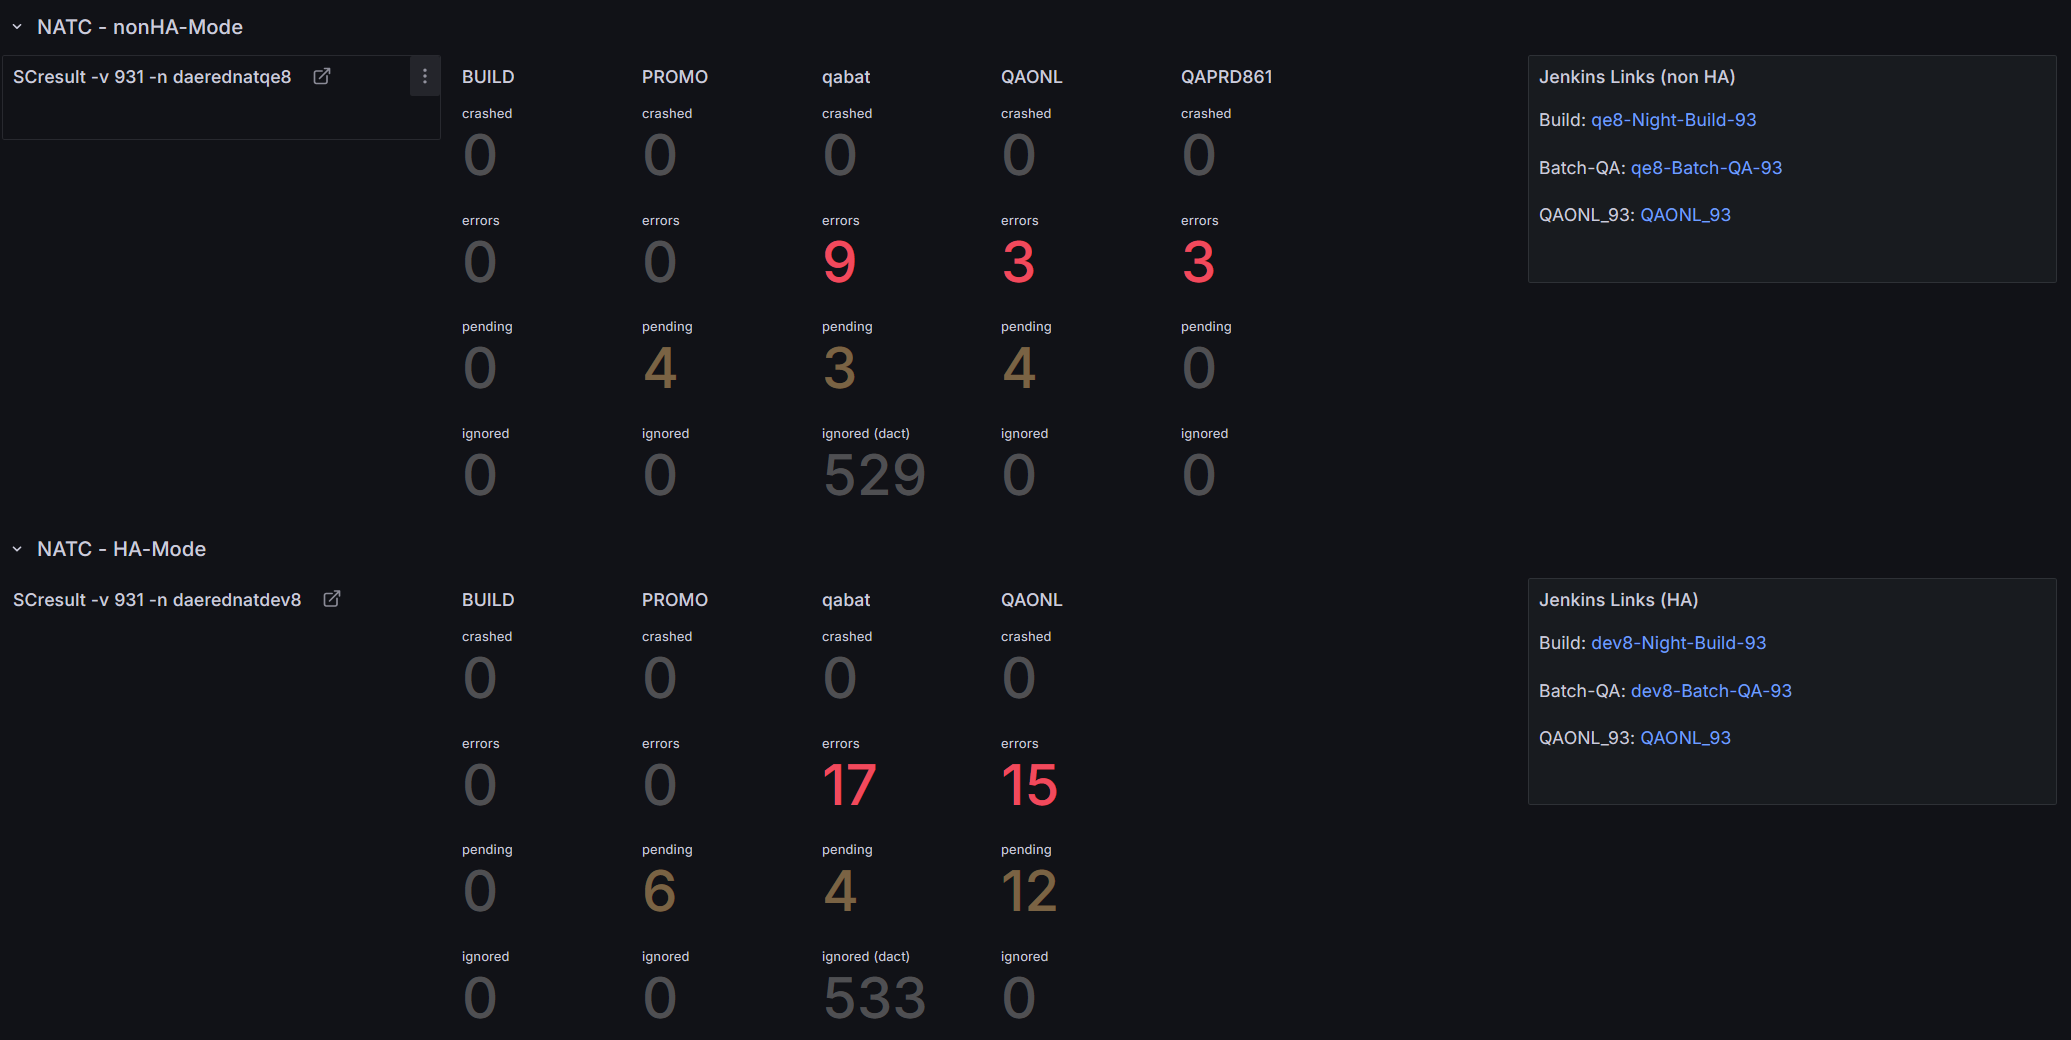
\includegraphics[width=1\linewidth]{Dashboard/20250704_DB_dev.png}
    \caption{Aufbau des gebauten Dashboard \textcolor{red}{(Ersetzen durch zensiertes Bild)}}
    \label{fig:aufbau_dashboard}
\end{figure}

% *****************************************************************
\section{technische Umsetzung des Datenflusses zur Dashboardanzeige}
\begin{figure}[H]
    \centering
    
\includegraphics[width=0.5\linewidth]{Dashboard/Grafana version.png}
    \caption{Grafana-Version}
    \label{fig:grafana_version}
\end{figure}
\chapter{Ergebnisse}
\label{ch:Ergebnisse}
Hier stehen Ergebnisse

\section{Usability Test}
\section{Nutzerbefragung}

\section{Zusammenfassung}
...
\chapter{Diskussion}
\label{ch:Diskussion}

Normalverteiltes Ergebnis\cite{normalverteilung_rechner}

% **********************************************************************************
% Auswertung des Usability-Tests
% **********************************************************************************
- Auswertung der Ergebnisse des Usability Tests in Bezug auf die funktionelle Eignung und Effizienz des Dashboards im Vergleich zum Legacy-System
-> Analyse der Erfüllung der Funktionsanforderungen des entwickelten Dashboards
-> Bewertung der Effizienz des Dashboards durch Gegenüberstellung der Testergebnisse

% **********************************************************************************
% Auswertung der Nutzerbefragung
% **********************************************************************************
- Auswertung der Ergebnisse der Nutzerbefragung zur Validierung der Testergebnisse sowie der Bewertung der User-Experience des Dashboards
-> Gegenüberstellung der Befragungsergebnisse des Legacy-Systems und Dashboards zur Validierung der vorangegangenen Dashboardbewertung
-> Auswertung der Nutzerbefragung zur Bewertung der User-Experience des Dashboards


% **********************************************************************************
% Methodenkritik zum Dashboard als Modernisierungslösung
% **********************************************************************************
Kritische Auseinandersetzung mit der verwendeten Methodik zur Modernisierung von Legacy-Systemen

% **********************************************************************************
% Methodenkritik zur Validierung
% **********************************************************************************
Kritische Auseinandersetzung mit der verwendeten Methodik zur Validierung der gewählten Dashboard-Lösung

% **********************************************************************************
% Abschließende Bewertung / Zusammenassung
% **********************************************************************************
Abschließende Bewertung der Dashboard-Lösung zur Modernisierung eines Legacy-Systems
\chapter{Schlussfolgerungen, Limitationen und Ausblick} % 5-10%
\label{ch:Fazit}

% In der Diskussion/im Fazit bzw. Schlussteil der Arbeit
%• gilt es, die empirischen Ergebnisse mit dem bereits vorgestellten Forschungsstand in Beziehung zu setzen. Wo decken oder widersprechen sich Ergebnisse? Welche Fragen sind offen geblieben?
%• Welche weiterführenden Fragen/Forschungsbedarf oder ggf. Handlungsempfehlungen für die Praxis lassen sich formulieren?

% FF: Wie sinnvoll ist die Einführung eines modernen Dashboards im Hinblick auf das Ziel, den Legacy-Testpoolmonitoring-Prozess effizienter und nutzerfreundlicher zu gestalten?


% Aufgreifen der Zielsetzung
\textcolor{red}{TODO: EInleitungssatz -} In einer Welt voller Altsysteme, hatte ich xy vor ...\\
Um einen Beitrag zu nachhaltigen und effizienten Systemen beizutragen, sollte mit dieser Forschungsarbeit herausgestellt werden, welchen Beitrag moderne Dashboards zur Modernisierung beitragen können eine geeignete Lösung darstellen. Dafür wurde anhand eines Legacy-Testpools ein Altsystem derer Ergebnisanzeige als Grundlage für ein neues Dashboard aufgegriffen. Ziel war es herauszustellen, wie sinnvoll dessen Einführung ist, um den Monitoring-Prozess effizienter und nutzerfreundlicher zu gestalten.

% Zusammenfassung
\section{Zusammenfassung der wichtigsten Ergebnisse}

Hierfür wurde eine Nutzerstudie bestehend aus einem Usability-Test und einer dazugehörigen Nutzerbefragung durchgeführt. Während die Nutzerbefragung auf den Prinzipien der ISO 9241-110 basiert, wurden innerhalb des Usability-Tests die nachträglich abgefragten Eigenschaften eingebaut. Auf dieser Grundlage konnten die beide Systeme anhand der drei Usability-Dimensionen Effektivität, Effizienz und Nutzerzufriedenheit verglichen werden.

Anhand dieser Forschungen konnten einige Möglichkeiten festgestellt werden.

Mithilfe der gewählten Dashboard-Lösung, ist ein zeitlich effizienteres Monitoring möglich als zuvor. Zwar wies der Usability-Test an dem Dashboard eine höhere Fehlerquote auf, als an dem Altsystem, jedoch liegt dies an der exzellenten Kenntnis der Nutzer des Altsystems sowie der Tatsache, dass die neue Lösung erst mit der Teilnahme an der Studie vorgestellt wurde. Allerdings konnte das Dashboard in den relevanten Stellen des Tests durch seine verbesserte Effektivität überzeugen und somit eine knapp 50\% bessere Effizienz vorweisen.

Anhand der regen Teilnahme an der Feedbackrunde war festzustellen, dass durchaus Verbesserungspotenzial an dem neuen Prototypen besteht. Jedoch wird damit auch Interesse auf Nutzerbasis gezeigt, dieses Projekt weiter zu fördern. Insgesamt sind die Nutzer auch viel zufriedener mit der Umsetzung und Nutzbarkeit des Dashboards, als mit der gewachsenen Altlösung.

% Einordnung in den aktuellen Forschungsstand
\section{Einordnung in den aktuellen Forschungsstand}

Die Dashboard-Lösung bildet eine nicht-invasive, risikoarme Modernisierungsmethode. Es hilft Anwendern Monitoring-Prozesse effizienter zu gestalten, da es die alten Strukturen in eine nutzerfreundliche Oberfläche verpackt. Da diese Dashboard-Lösung jedoch keine bestehenden Strukturen entfernt, entsteht auch keine Hürde für ältere Mitarbeiter, welche potenziell Probleme mit der Umstellung haben.

Weiterhin bietet es sich an, eine Ergebnisanzeige so zu modernisieren, um vergessene oder geduldete Altlasten aufzudecken. Da es sich teilweise schwierig gestaltet, diese durch die Modernisierungsmaßnahme automatisiert auszulesen, bietet der Prozess eine geeignete Gelegenheit, die Altlasten neu zu entdecken und aufzuarbeiten.

Es bietet darüber hinaus die Gelegenheit, auf das Thema der Modernisierung aufmerksam zu machen, wie diese beispielsweise eine zur Optimierung von Prozessen eingesetzt werden kann. Das Dashboard kann somit als eine geeignete Modernisierungsmethode für Legacy-Anwendungen mit Ergebnisanzeige eingeordnet werden.

% Grenzen + mögliche Weiterentwicklungen
\section{Grenzen des entwickelten Prototypen und mögliche Weiterentwicklungen}

Da die Dashboard-Lösung bislang ein Projekt prototypischen Charakters ist, kann dieses Projekt noch stark ausgeweitet werden. Neben dem Ausbau auf den restlichen Testpool, kann das bereits genannte Nutzerfeedback zur Optimierung angewendet werden. Dieses liefert hilfreiche Hinweise bezüglich dem bestehenden Workflow sowie Formatierung, Größe und Kapselung zusammengehöriger Informationen, um den Übergang auf das neue System zu erleichtern.

Bisher bietet das Dashboard zudem rein informell betrachtet keinen Mehrwert. Da die Daten unabhängig vom bestehenden System ausgewertet und aufgearbeitet werden, sind vorgeschlagene Features wie die Darstellung der Fehlerwerte der letzten zwei Wochen in einem Verlaufsdiagramm möglich. Da das Dashboard jeden Tag überwacht wird, ist ein direkter Vergleichswert zum Vortag denkbar. Dieser zeigt zusätzlich zur Fehlerzahl, ob und wie viele Fehler mehr oder weniger als am Vortag vorliegen.

Da das System keine Veränderung am Altsystem vornimmt, kann diese Lösung ausschließlich als erster Schritt des Modernisierungsprozesses angesehen werden. Es hilft Altlasten zu erkennen und fachfremden Personen den Einstieg in das System zu erleichtern. Ein nächster Schritt wäre, diese Erkenntnisse zur Umstrukturierung und Optimierung oder zur Umstrukturierung in Kombination mit einem Rehosting auf zum Beispiel ein standardisiertes, modernes Framework zu nutzen.

% Ausblick + Empfehlungen für weitergehende Forschung
\section{Ausblick und Empfehlungen für weitergehende Forschung}

Dieses Prototyp-Projekt kann in naher Zukunft mit den aufgezählten Features und vorgeschlagenen Verbesserungen ausgebaut und optimiert werden.
Dabei können die Erkenntnisse aus dieser Forschungsarbeit eine Grundlage für beispielsweise folgende Aufbaustudien bieten:

Aufgrund der begrenzten Kapazitäten ist eine Wiederholung des Versuchs mit einer höheren Teilnehmerzahl, oder  einem größeren Umfang in Funktionalität und Aufgaben denkbar, um die Ergebnisse mit einer größeren Teststärke validieren zu können.
Mit mehr Teilnehmern einer Studie kann auf eine breitere Fächerung sowie gleichmäßigere Verteilung der Nutzer in Erfahrungslevel, Expertise sowie Altersklasse geachtet werden. Dies ermöglicht, Rückschlüsse auf die verschiedenen Variablen ziehen zu können. Dieser Ansatz kann Erkenntnisse darauf bieten, wie Modernisierungsmaßnahmen aufgefasst werden oder wie diese in den verschiedenen Nutzergruppen angegangen werden sollten.

Eine weitere Möglichkeit stellt die Untersuchung tiefergreifender Modernisierungsmaßnahmen wie der Umstrukturierung oder des Rehostings dar. Es könnten verschiedene Ansätze getestet oder unterschiedliche standardisierte Frameworks miteinander verglichen werden, um eine gute Lösung für das jeweilige System finden zu können.

\textcolor{red}{TODO: brauche ich einen weiteren Abschlusssatz?}

% -> was ist meine Empfehlung (potenzielle neue Arbeiten) die ich gebe, damit diese Forschung in der Zukunft eingesetzt werden kann



%*************************************************************************
% Recommendations
%*************************************************************************
%\part{Empfehlungen zur Erstellung wissenschaftlicher Abschlussarbeiten}
%\label{pt:recommendations}

%*************************************************************************
% Backmatter
%*************************************************************************
%\renewcommand{\thechapter}{\alph{chapter}}
\appendix
\cleardoublepage
\part{Appendix}

\chapter{\textcolor{Salmon}{Überblick über die aktuelle Studienlage}}
\label{ch:SdF:sec:Studienlage}

\textcolor{red}{Muss aus Platzgründen vermutlich in den Anhang verschoben werden}

\noindent
Suchbegriffe \url{https://scholar.google.com}\\
- dashboard\\
- modernizing test infrastructure\\

\noindent
\textcolor{red}{vielversprechend: noch nicht final erkundet:}
\begin{itemize}
    \item \url{https://www.researchgate.net/profile/Jeffrey-Ogeawuchi/publication/391986603_Revolutionizing_Business_Intelligence_Reporting_Advances_in_Cloud-Native_Data_Visualization_Tools_for_Real-Time_Insights/links/684dcb89df3fa4286a40c539/Revolutionizing-Business-Intelligence-Reporting-Advances-in-Cloud-Native-Data-Visualization-Tools-for-Real-Time-Insights.pdf} (2023)
    \item \url{https://yadda.icm.edu.pl/baztech/element/bwmeta1.element.baztech-662d6498-ed06-4ef9-a18b-388b7da69021} (2020)\\
          \url{https://managementpapers.polsl.pl/wp-content/uploads/2020/05/143-Zdonek-2.pdf}
    \item \url{https://f.hubspotusercontent30.net/hubfs/6618383/Report%20-%20TDWI%20Best%20Practices%20-%20Q4-2021.pdf} (Report 2021, S. 6)
    \item \url{https://eprints.qut.edu.au/66731/} (2012)\\
          \url{https://eprints.qut.edu.au/66731/1/DA_Daniel_Filonik.pdf}
    \item \url{https://oulurepo.oulu.fi/bitstream/handle/10024/57322/nbnfioulu-202506194837.pdf?sequence=1} (June 2025, Master Thesis)
    \item \url{https://ajates-scholarly.com/index.php/ajates/article/view/6} (Feb 2025)
          \url{https://ajates-scholarly.com/index.php/ajates/article/view/6/7}
          \url{https://doi.org/10.63125/cqm5jk84}
\end{itemize}

\noindent
\textcolor{red}{weitere - noch nicht final erkundet}
\begin{itemize}
    \item \url{https://www.sciencedirect.com/science/article/abs/pii/S138650561830131X?via%3Dihub} (2018)
    \item \url{https://ieeexplore.ieee.org/abstract/document/7579419/metrics#metrics} (2016)
    \item \url{https://pubmed.ncbi.nlm.nih.gov/27441717/} (2016)\\
          \url{https://www.liebertpub.com/doi/10.1089/big.2015.0059} (2016, anderer Link)
    \item \url{https://www.sciencedirect.com/science/article/abs/pii/S1045926X18301009?via%3Dihub} (2019)
    \item \url{https://docs.media.bitpipe.com/io_13x/io_133039/item_1388007/Data%20Warehouse%20Modernization.pdf} (Report 2016)
    \item \url{https://aaltodoc.aalto.fi/items/1f03f049-5d3b-441d-ba30-777d7bbe2b54} (2017, Master Thesis)\\
          \url{https://aaltodoc.aalto.fi/server/api/core/bitstreams/1f040936-3eb3-46a5-85dd-d9f8140310fd/content}
    \item \url{https://papers.ssrn.com/sol3/papers.cfm?abstract_id=5047056} (Jan, 2025)\\
          \url{https://papers.ssrn.com/sol3/Delivery.cfm/5047056.pdf?abstractid=5047056&mirid=1&type=2}
    \item \url{https://www.osti.gov/biblio/1358407} (2016)
\end{itemize}

\chapter{Anforderungstabellen nach ISO 9241-110}

include Bilder je Kategorie - für altes und neues System
\label{fig:Anforderungskatalog_ISO_alt}
\label{fig:Anforderungskatalog_ISO_neu}
\chapter{Anhänge zum Dashboard}
\label{Add:Dashboard}

\section{Evalution zur Auswahl des Tools für das Dashboard}
\chapter{Mitschriften von Mitarbeiteraussagen während der Befragung und des Usability-Tests}
\label{Add:Mitschriften_Mitarbeiteraussagen}

\noindent
\textcolor{red}{TODO: Mitschriften der Diskussionsrunde rausschreiben / formatieren}

\begin{figure}
    \centering
    
\includegraphics[width=1\linewidth]{Anhänge/00_stockfoto.jpg}
    \caption{Mitschriften Mitarbeiteraussagen \textcolor{red}{TODO: aufarbeiten und einfügen}}
    \label{fig:Mitschriften_Mitarbeiteraussagen}
\end{figure}
\chapter{Anhänge zur Nutzerbefragung}
\label{Add:Pruemper}
\section{Abkürzungsverzeichnis der nachfolgenden ISO-Inter\-ak\-tions\-prinzipien}
\label{Add:Nutzerbefragung_Prümper:ISO-Abkürzungen}
Die Nachfolgenden Abkürzungen wurden aus \cite{Pruemper:Fragebogen-S:2006} übernommen:
\begin{itemize}
    \item aa: Aufgabenangemessenheit
    \item sb: Selbstbeschreibungsfähigkeit
    \item ek: Erwartungskonformität
    \item If: Erlernbarkeit
    \item sk: Steuerbarkeit
    \item ft: Robustheit gegen Nutzungsfehler
    \item Ik: Nutzerbindung
\end{itemize}

\section{Begründung zur Ausfilterung bestimmter Fragen aus dem Fragebogen \cite{Pruemper:Fragebogen-S:2006}}
\label{Add:Nutzerbefragung_Prümper:Begründung_Filterung}

Nachfolgend wird jeweils die positive Ausprägung der gefilterten Fragen aufgelistet.\\

\noindent
Beide Systeme ermöglichen eine einfache Ansicht von Informationen. Die individuelle Arbeitsweise von Personen zur Ansicht/Abarbeitung dieser Informationen, ist kein Bestandteil dieser Untersuchung.
Beide Systeme ermöglichen die benötigte Flexibilität. Daher wurden folgende Fragen aus der Nutzerbefragung entfernt:
\begin{itemize}
    \item Die Software erzwingt keine unnötig starre Einhaltung von Bearbeitungsschritten. (Sk1) % (Sw12)
    \item Die Software erzwingt keine unnötigen Unterbrechungen der Arbeit. (Sk3) % (Sw15)
    \item Die Software lässt sich von mir gut an meine persönliche, individuelle Art der Arbeitserledigung anpassen. (Ik2) % (Sw27)
    \item Die Software lässt sich - im Rahmen ihres Leistungsumfangs - von mir gut für unterschiedliche Aufgaben passend einrichten. (Ik3) % (Sw29)
\end{itemize}

\noindent
Es handelt sich für diesen Use-Case (Testpoolmonitoring) ausschließlich um die Ergebnis-Ansicht als Informationsquelle. Es können keine Eingaben getätigt werden. Interaktionen wie Erweiterung/Veränderung des Dashboards/der Ansicht oder weitere administrative Tätigkeiten, die das Framework Grafana ermöglicht, sind kein Teil der täglichen Aufgabe. Daher wurden folgende Fragen aus der Nutzerbefragung entfernt:
\begin{itemize}
    \item Die Software liefert in zureichendem Maße Informationen darüber, welche Eingaben zulässig oder nötig sind. (sb1) % (Sw08)
    \item Die Software bietet auf Verlangen situationsspezifische Erklärungen, die konkret weiterhelfen. (sb2) % (Sw09)
    \item Die Software informiert in ausreichendem Maße über das, was es gerade macht. (ek2) % (Sw18)
    \item Die Software liefert gut verständliche Fehlermeldungen. (ft1) % (Sw23)
    \item Die Software erfordert bei Fehlern im Großen und Ganzen einen geringen Korrekturaufwand. (ft2) % (Sw24)
    \item Die Software gibt konkrete Hinweise zur Fehlerbehebung. (ft3) % (Sw25)
    \item Die Software lässt sich von mir leicht erweitern, wenn für mich neue Aufgaben entstehen. (Ik1) % (Sw26)
\end{itemize}

\newpage
\section{gekürzter Fragebogen der Nutzerbefragung nach Prümper}
\label{Add:Nutzerbefragung_Prümper:gekürzter_Fragebogen}

%Folgende Fragen wurden übernommen: Sw02, Sw04, Sw05, Sw10, Sw13, Sw16, Sw20, Sw31, Sw33 und Sw35. (Reihenfolge abweichend)\textcolor{red}{\cite{https://inf-schule.de/content/9_software/1_gui/1_benutzerfreudlichkeit/3_uebungen/Methode_Isonorm-Fragebogen.pdf}}

Folgende Fragen wurden übernommen: aa1, aa2, aa3, sb3, sk2, ek1, ek3, If1, If2 und If3. (Reihenfolge abweichend) \cite{Pruemper:Fragebogen-S:2006}

\begin{figure} [H]
    \centering
    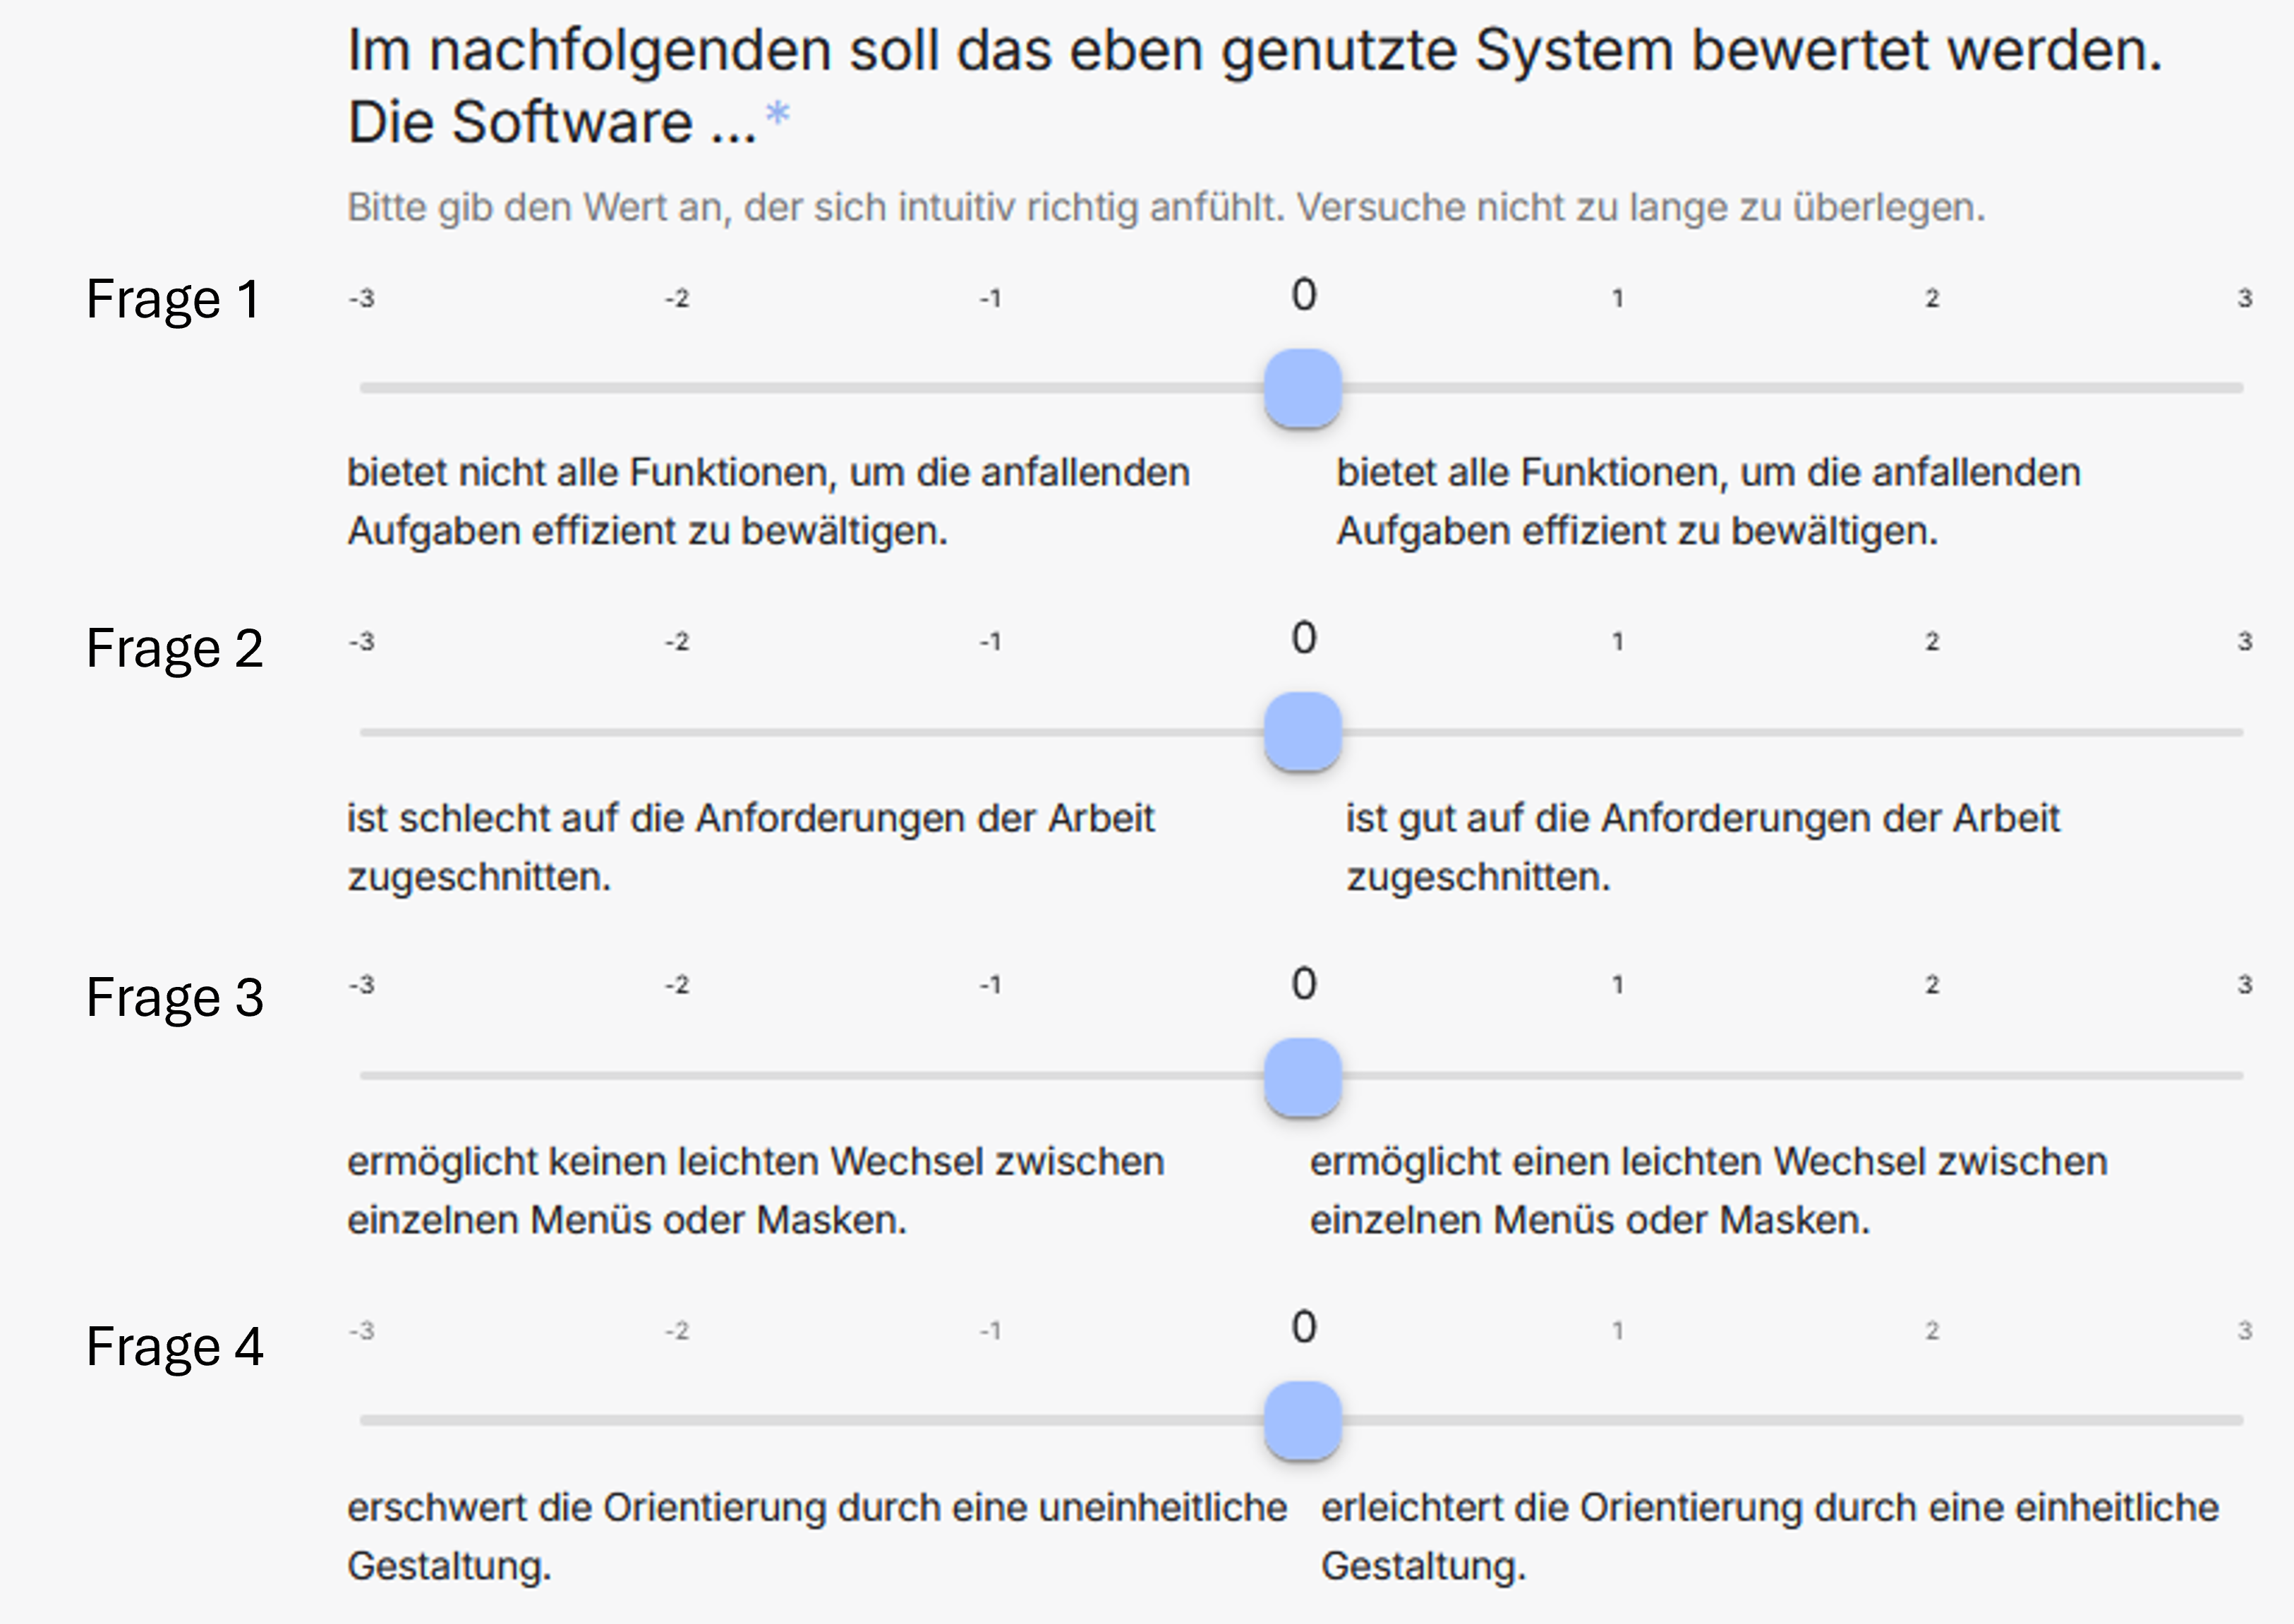
\includegraphics[width=0.85\linewidth]{Anhänge/Nutzerbefragung/Survio_Pruemper_1.PNG}
    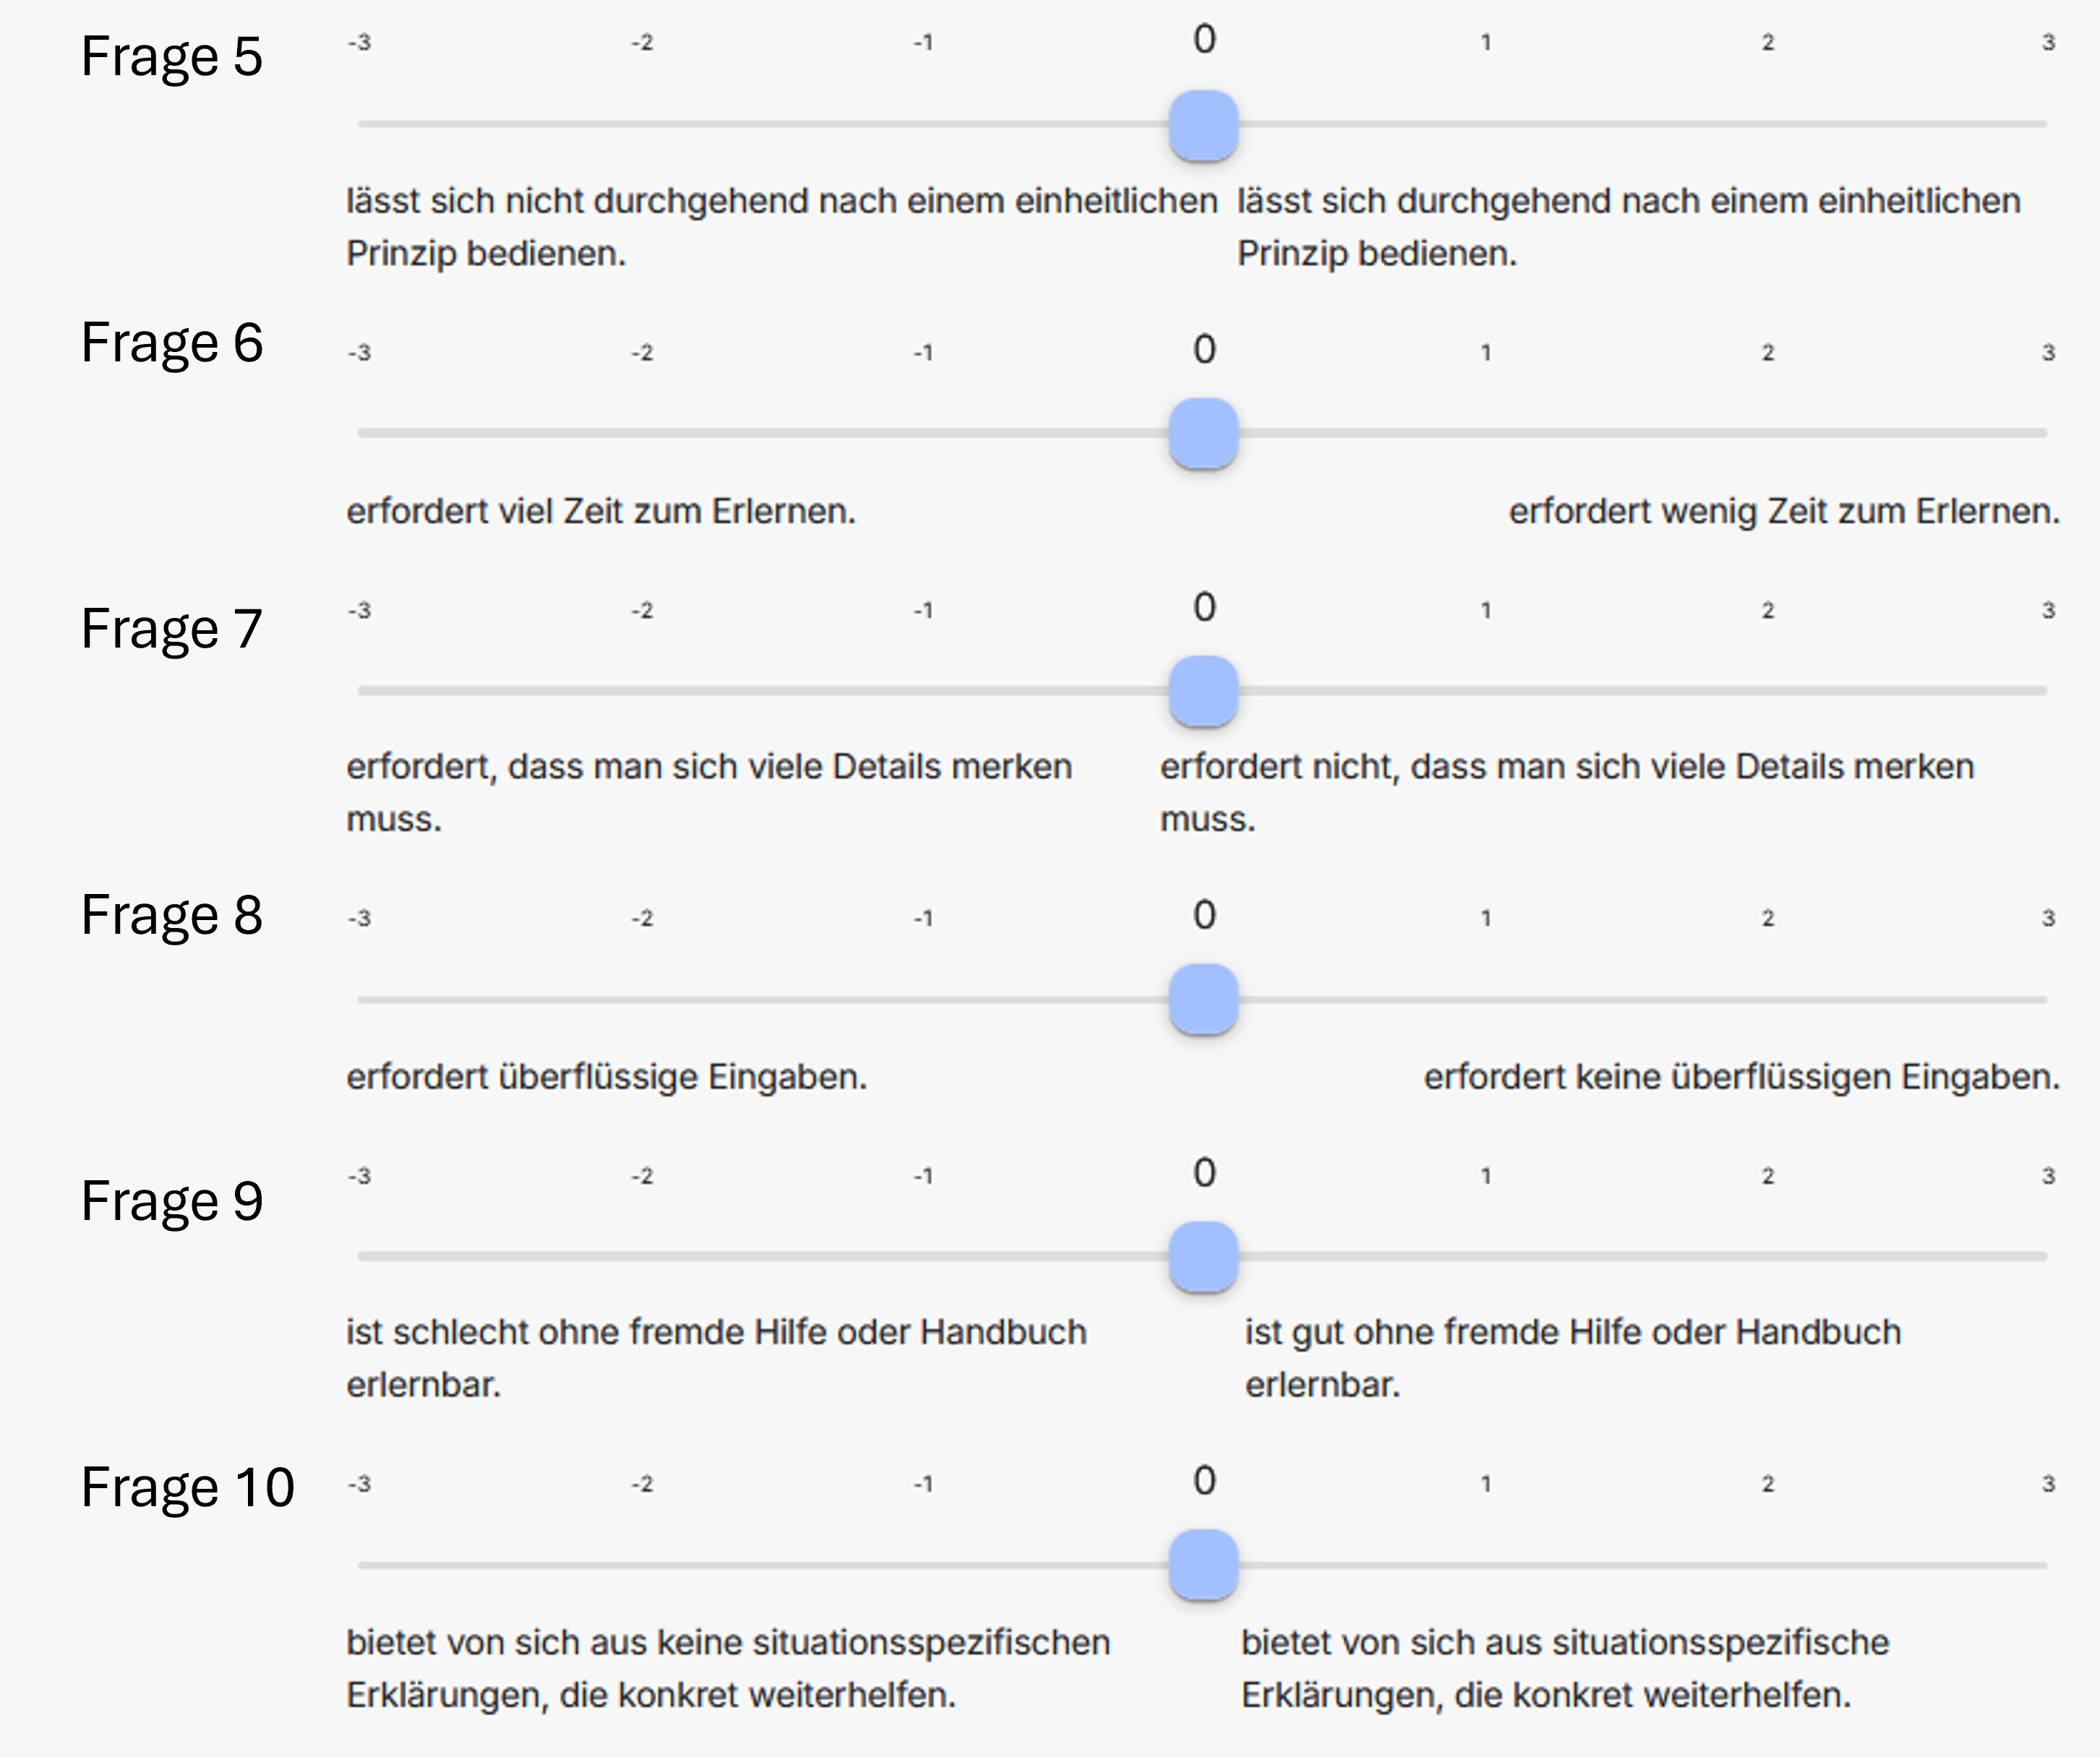
\includegraphics[width=0.85\linewidth]{Anhänge/Nutzerbefragung/Survio_Pruemper_2.PNG}
    \caption{gekürzter Fragebogen nach Prümper (Screenshot aus Survio)}
    \label{fig:fragebogen_prümper}
\end{figure}

\section{Tabellen mit rohen Daten}

\begin{table}[H]
    \centering
    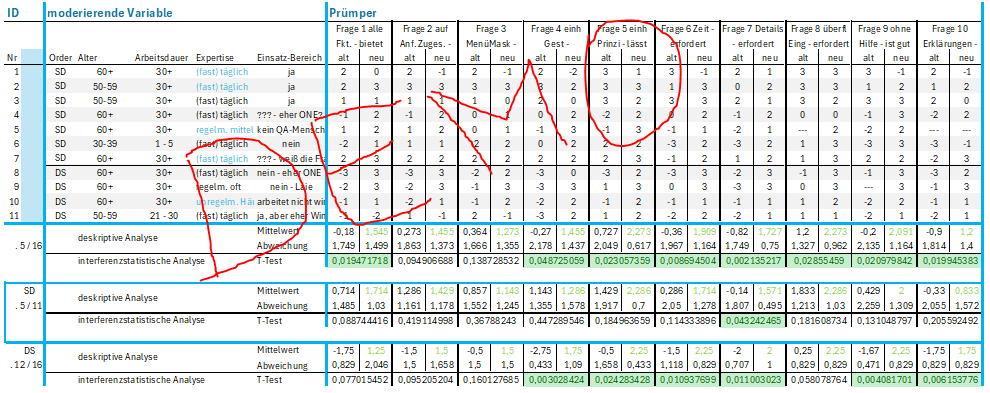
\includegraphics[width=0.65\textheight, angle=90]{Anhänge/Nutzerbefragung/prümper-Tabelle_demo.PNG}
    \caption{Nutzerbefragung nach Prümper - Tabellarische Daten}
    \label{tab:Nutzerbefragung:rohe_Daten}
\end{table}
\section{Histogramme der Differenzen}
\begin{figure}[H]
    \centering
    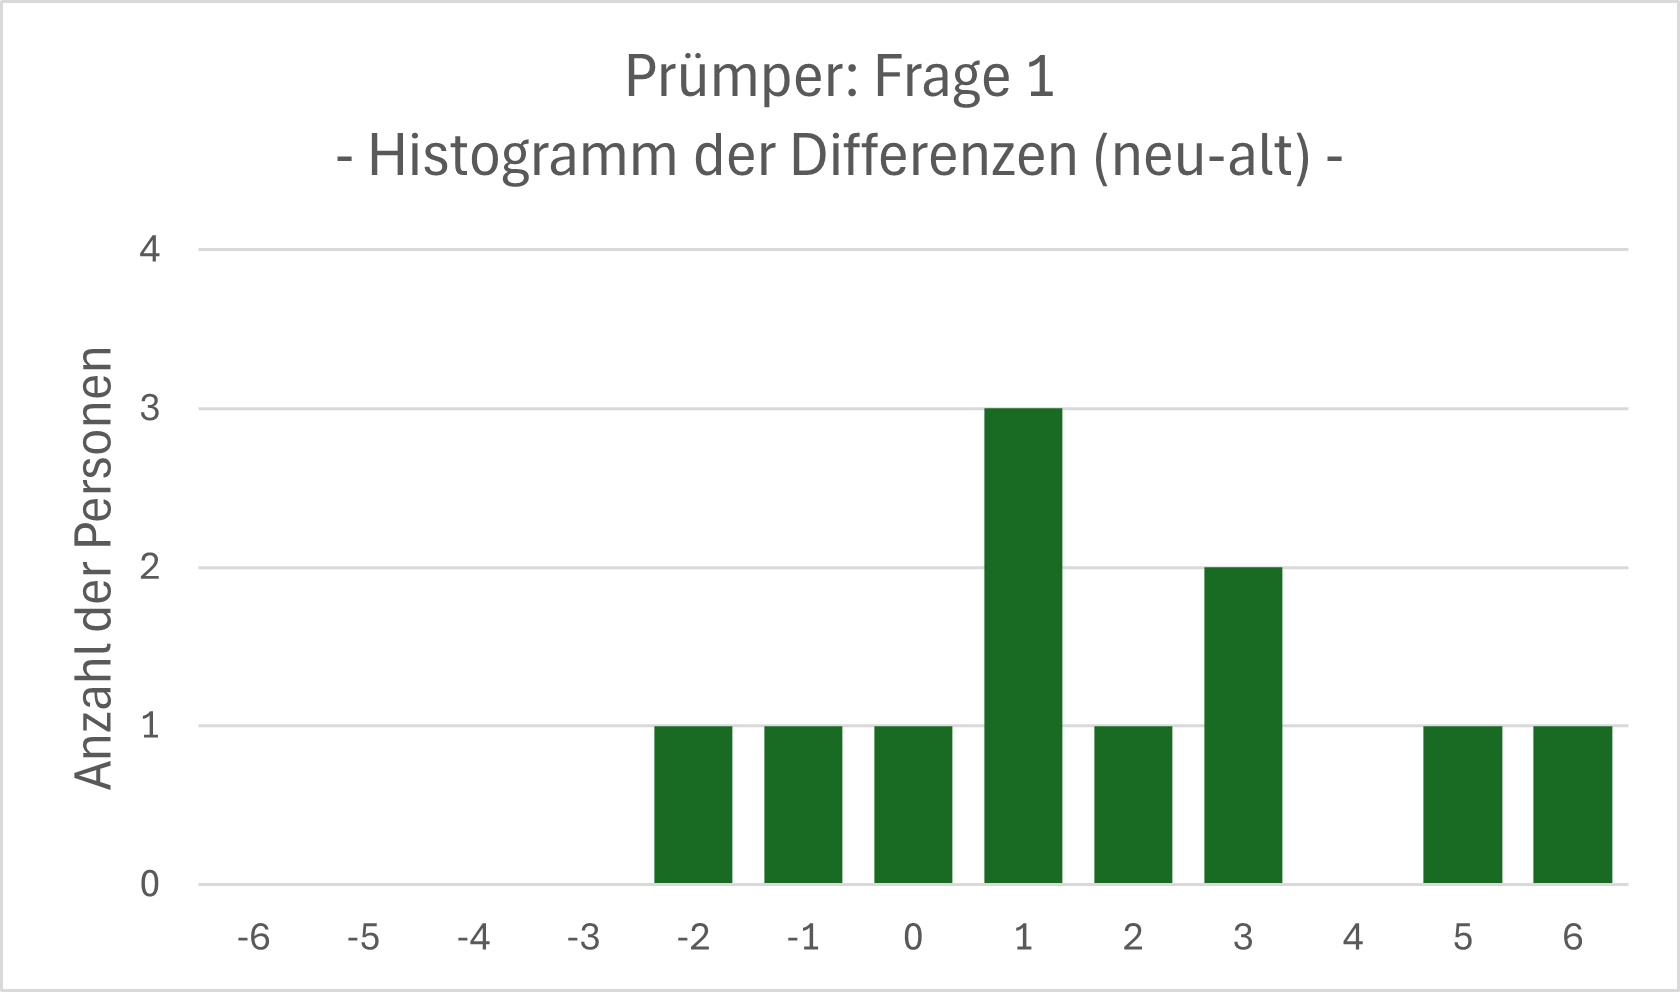
\includegraphics[width=0.45\linewidth]{Diagramme/hist_1_pruemper.png}
    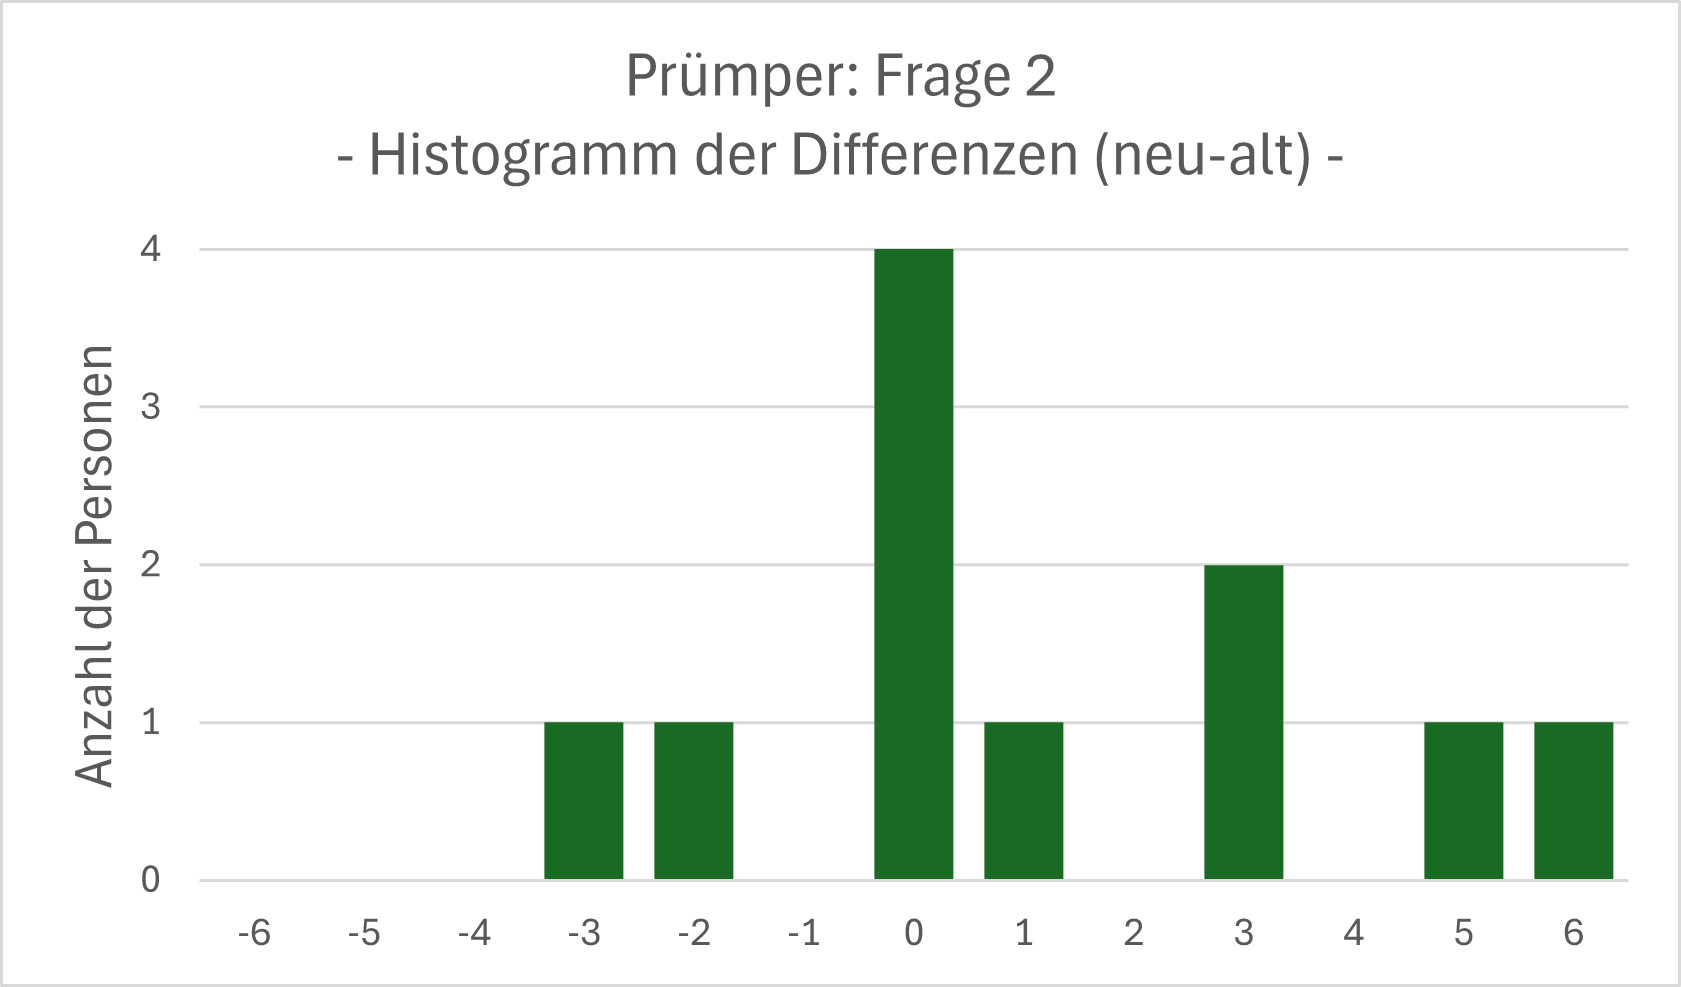
\includegraphics[width=0.45\linewidth]{Diagramme/hist_2_pruemper.png}
    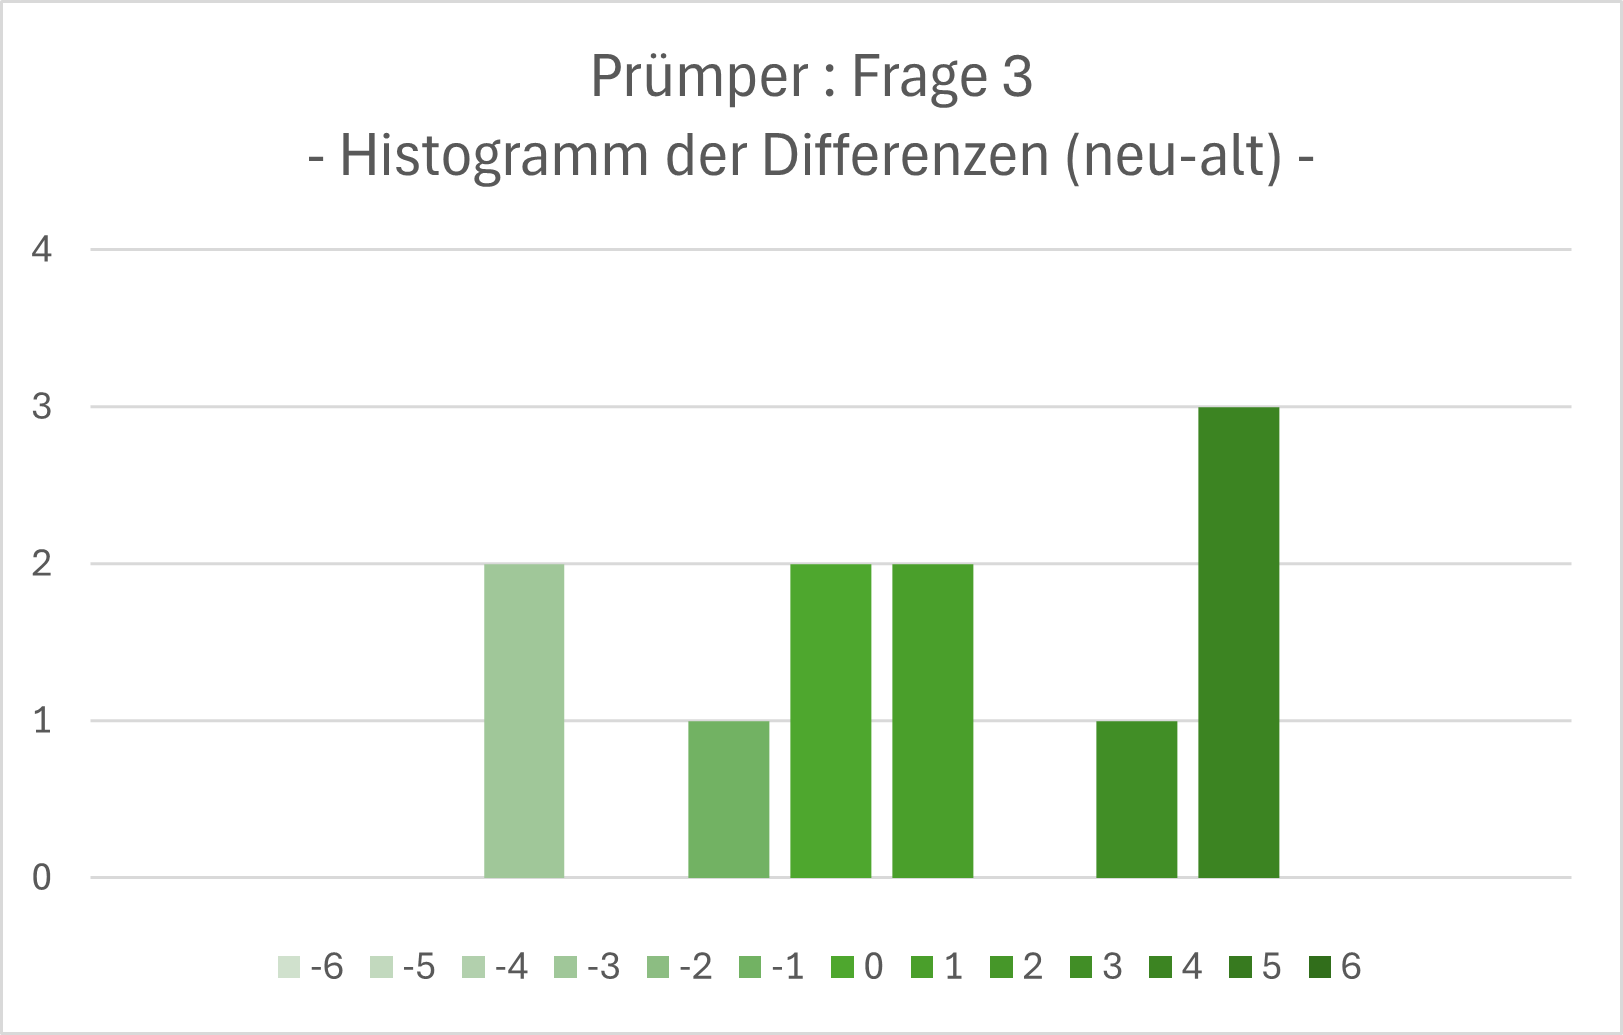
\includegraphics[width=0.45\linewidth]{Diagramme/hist_3_pruemper.png}
    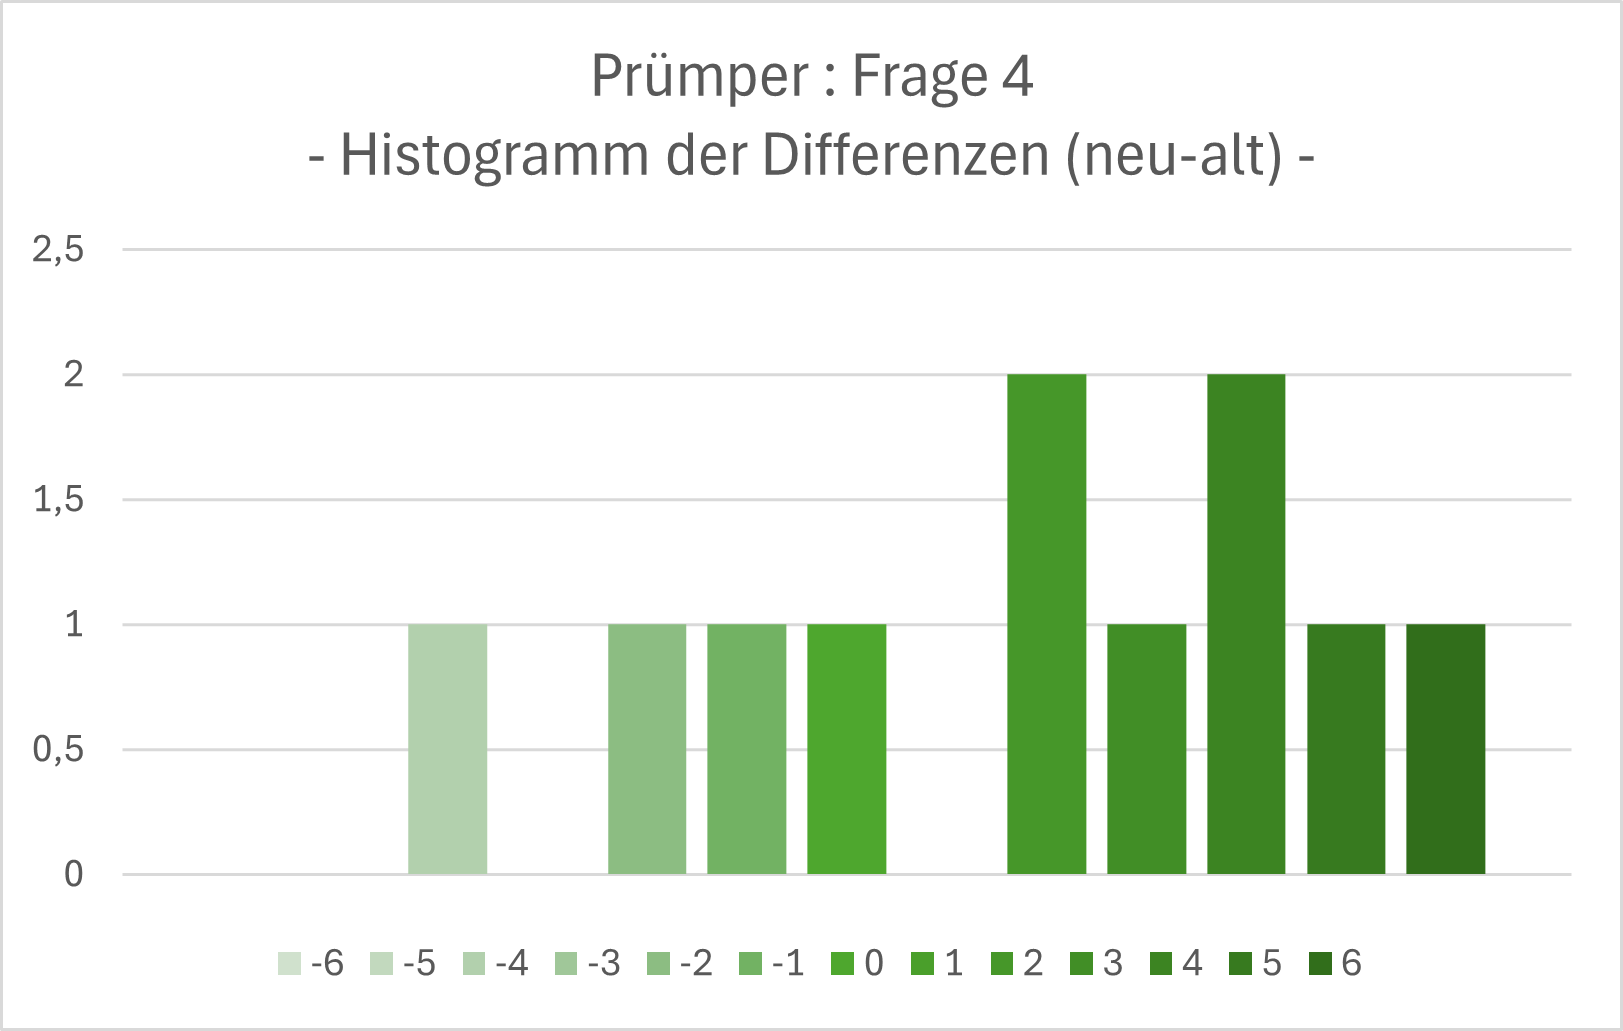
\includegraphics[width=0.45\linewidth]{Diagramme/hist_4_pruemper.png}
    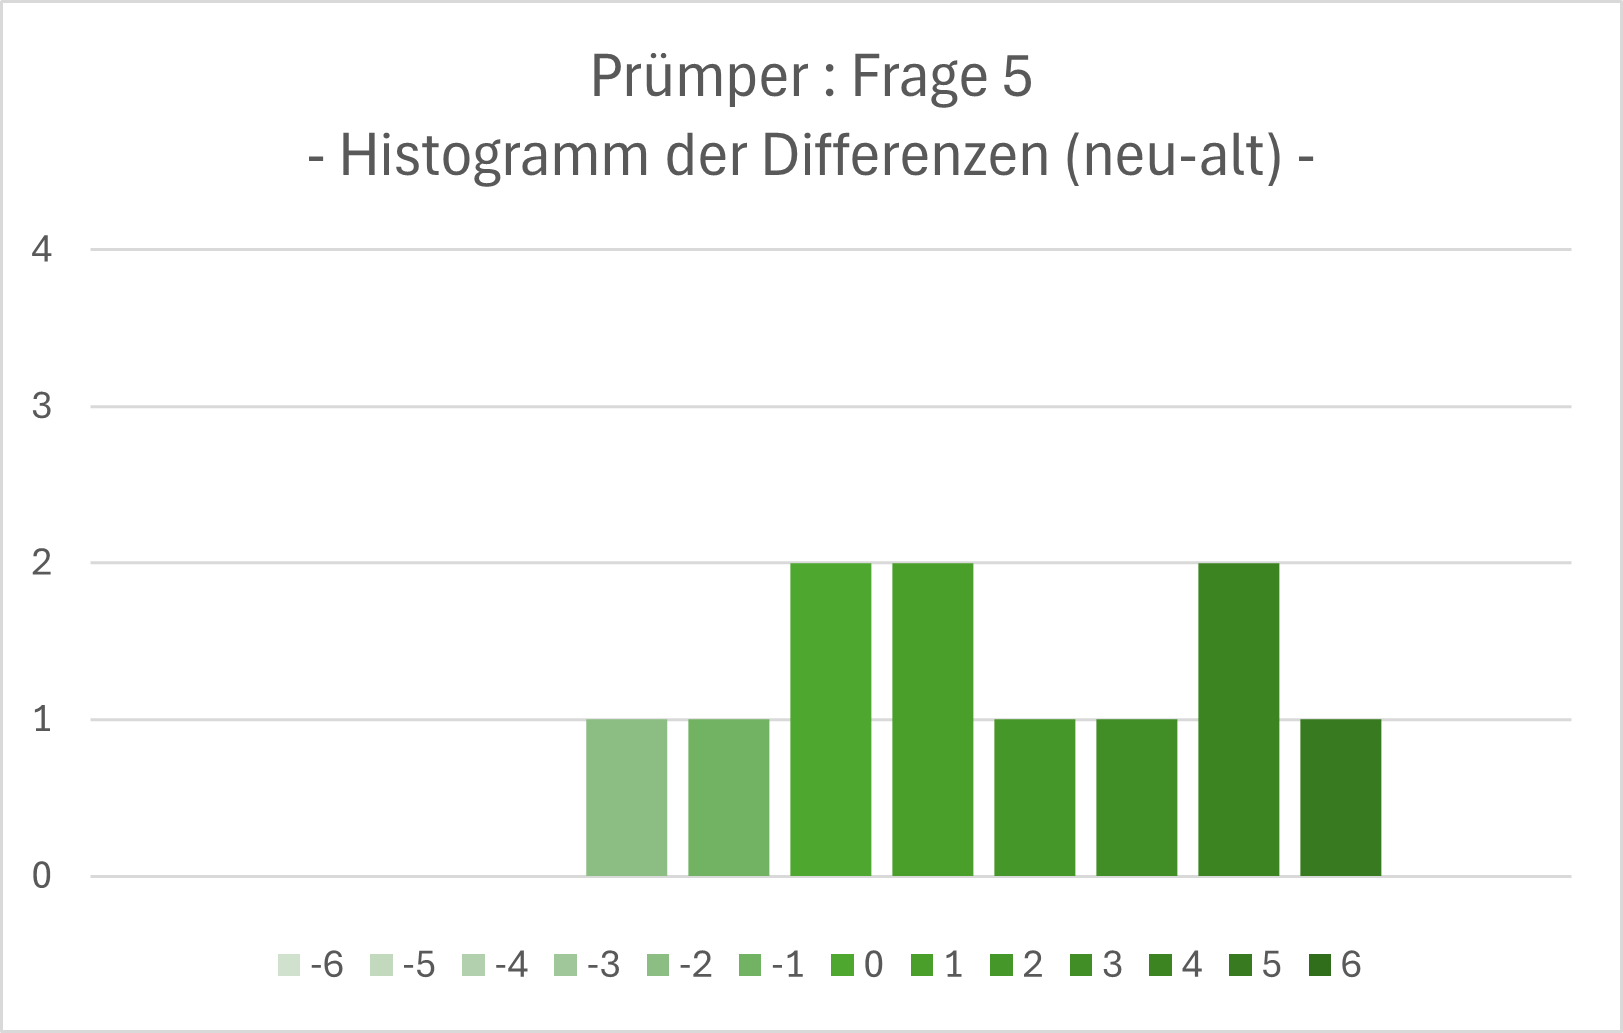
\includegraphics[width=0.45\linewidth]{Diagramme/hist_5_pruemper.png}
    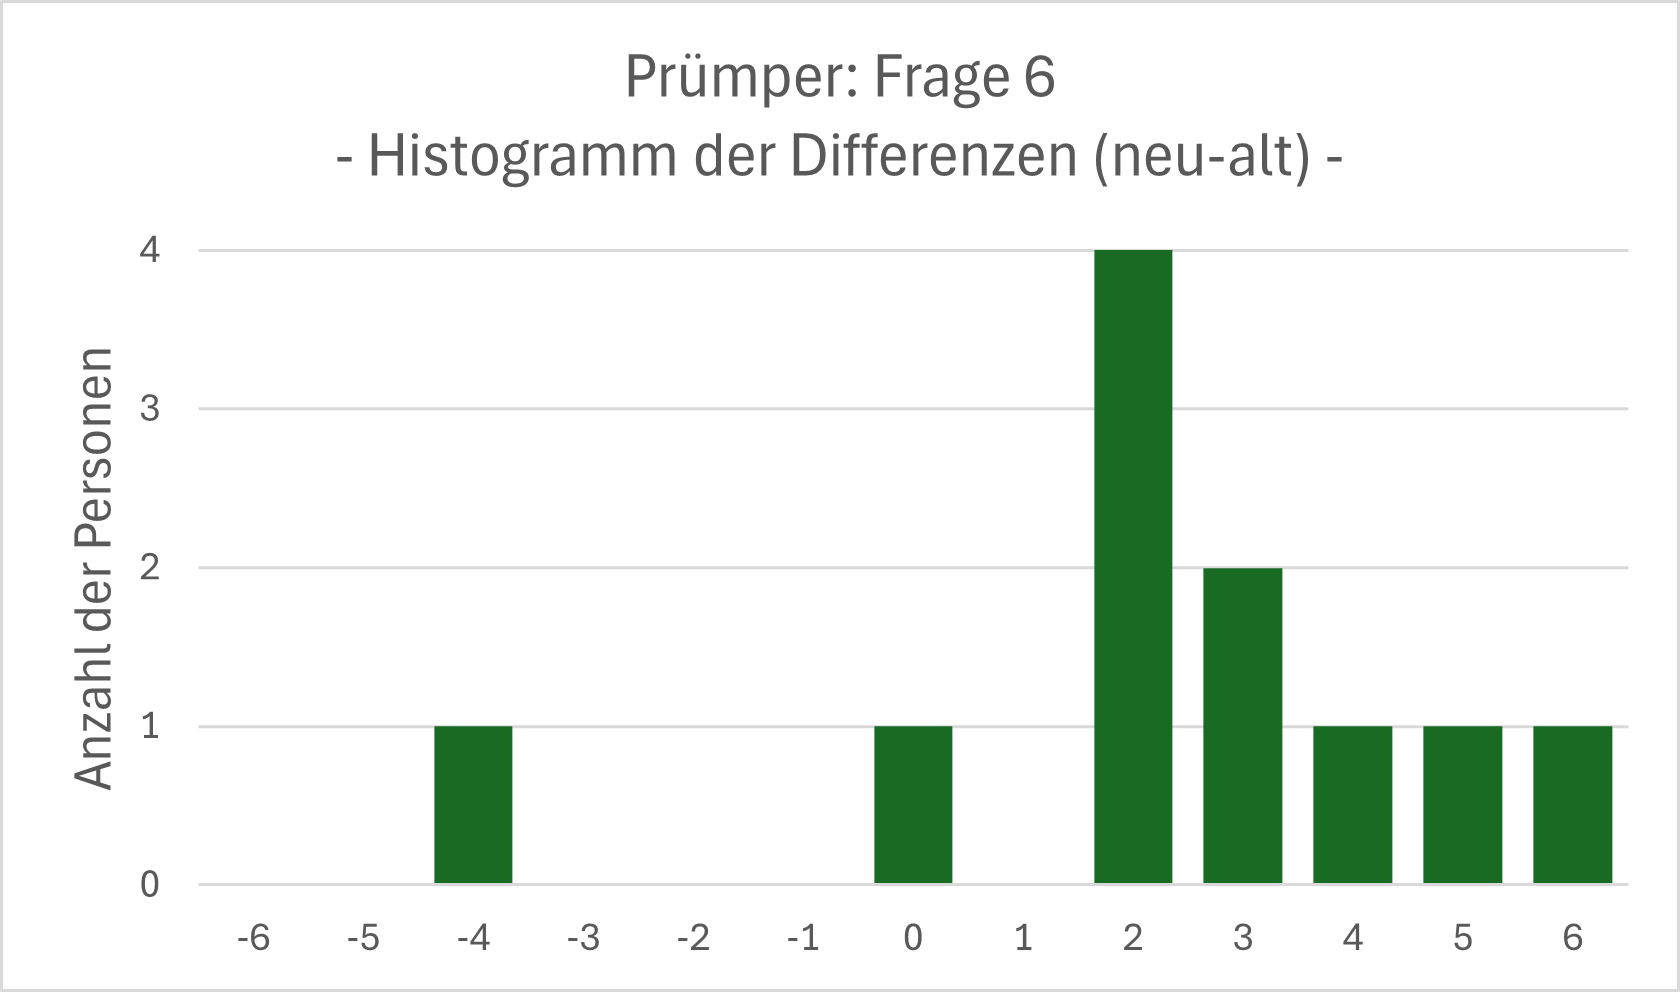
\includegraphics[width=0.45\linewidth]{Diagramme/hist_6_pruemper.png}
    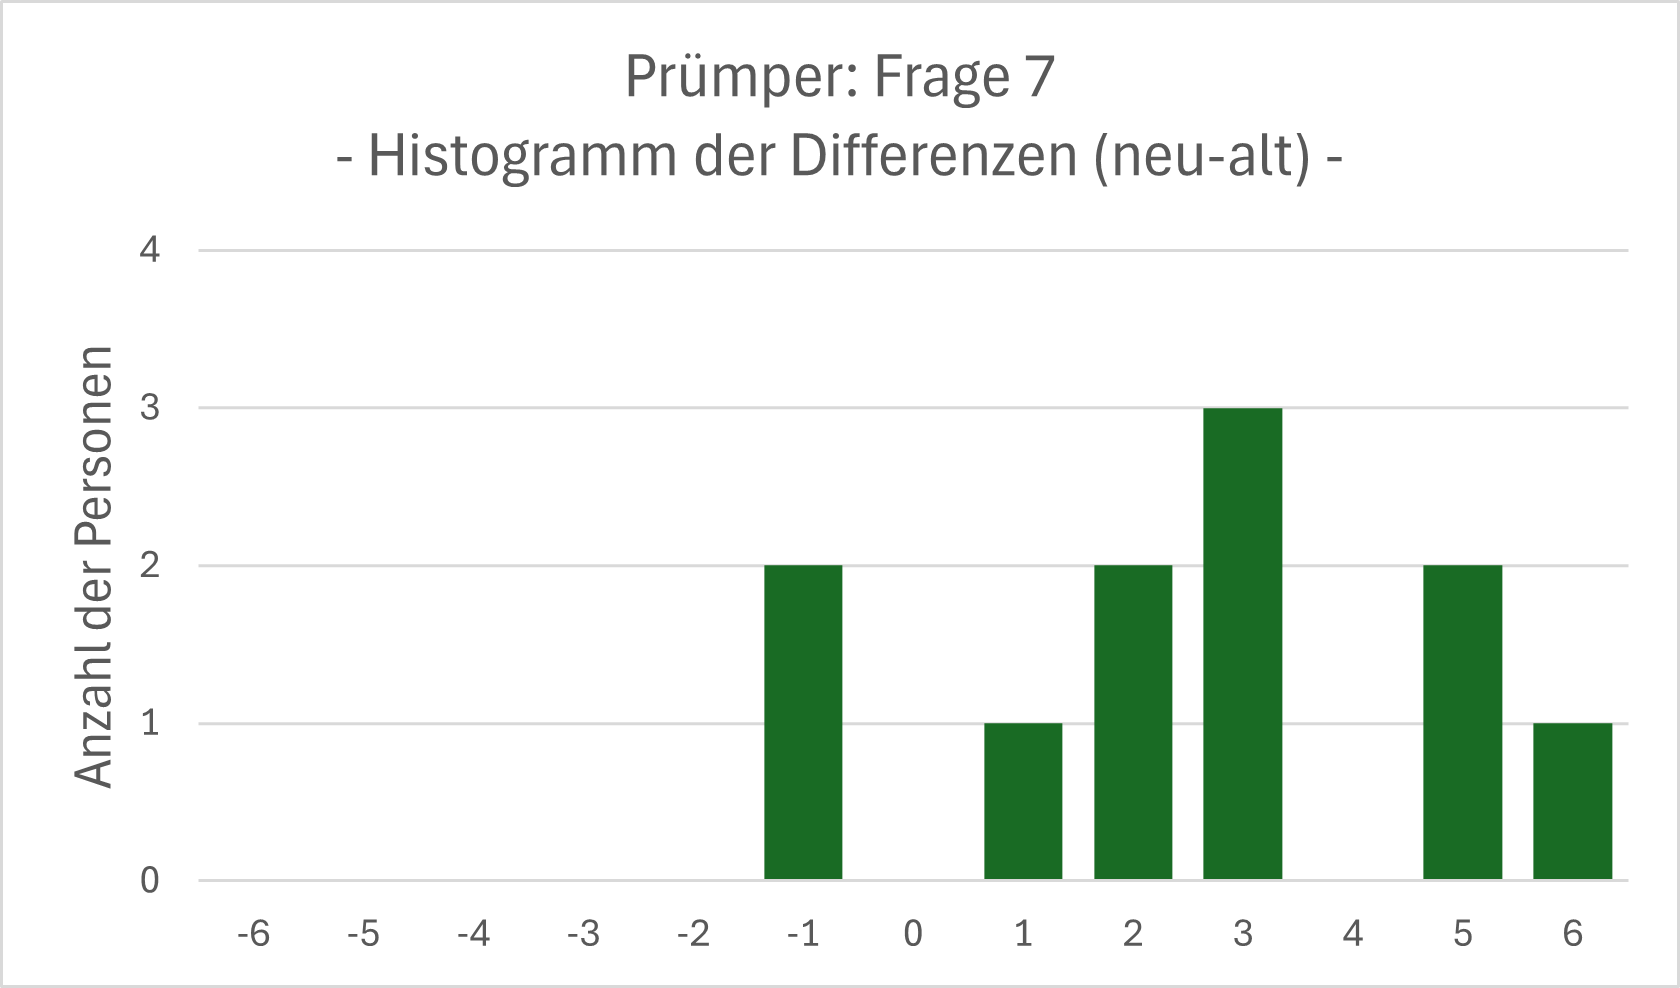
\includegraphics[width=0.45\linewidth]{Diagramme/hist_7_pruemper.png}
    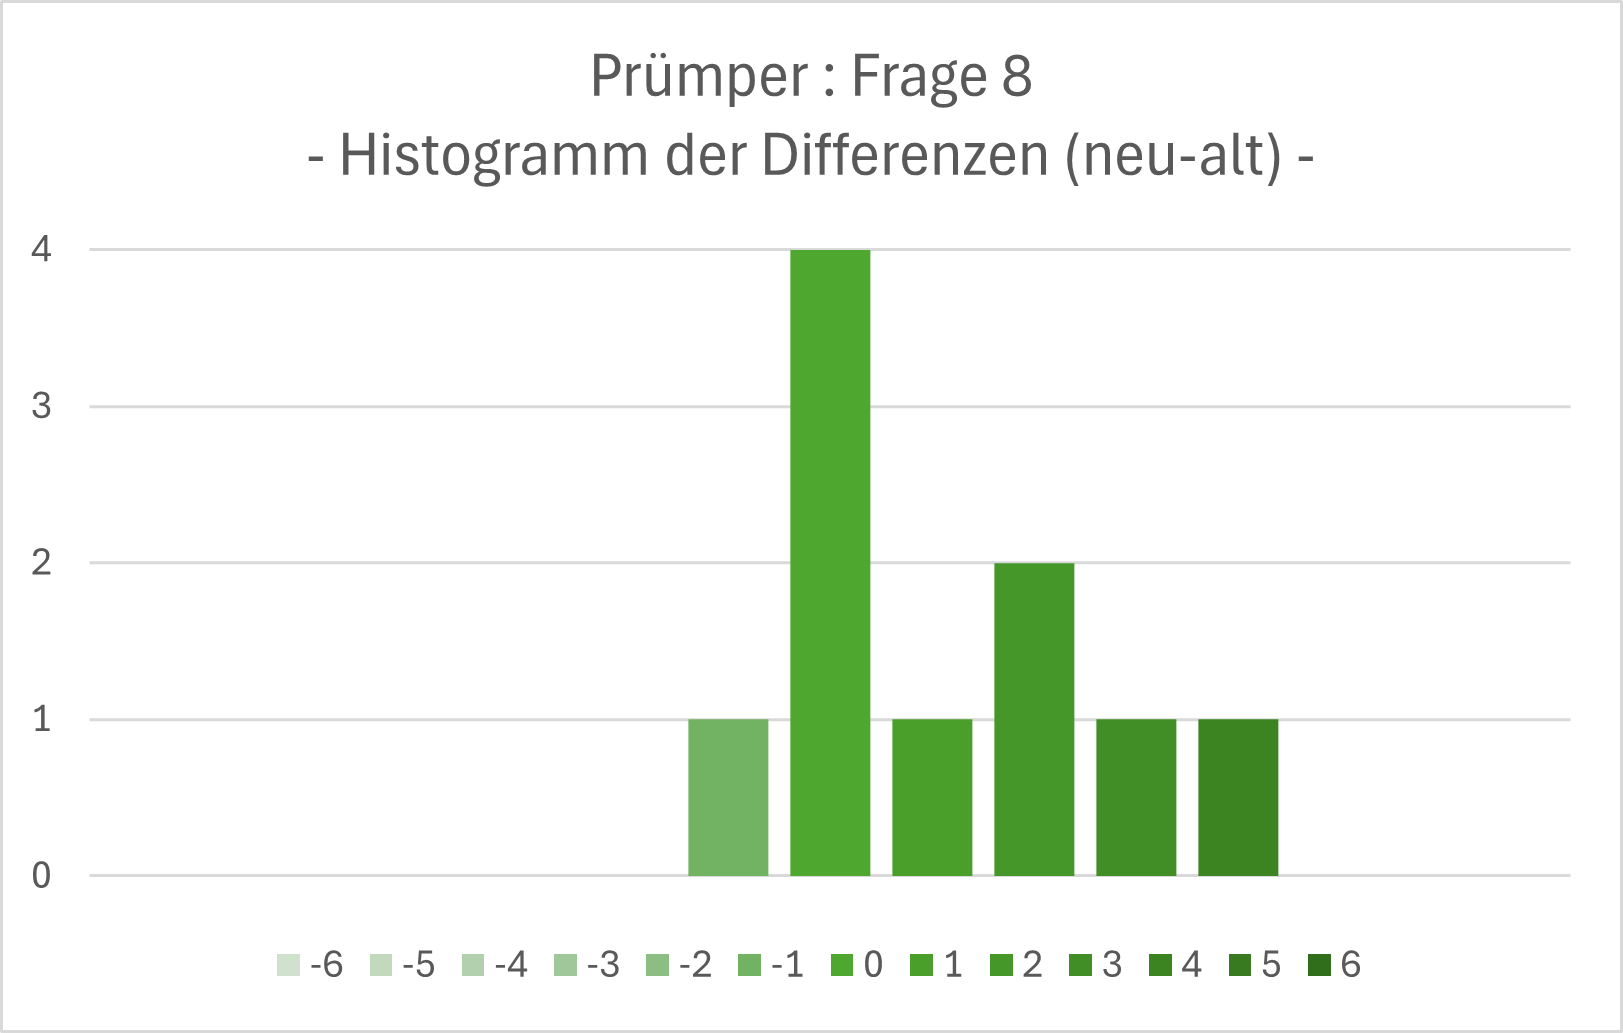
\includegraphics[width=0.45\linewidth]{Diagramme/hist_8_pruemper.png}
    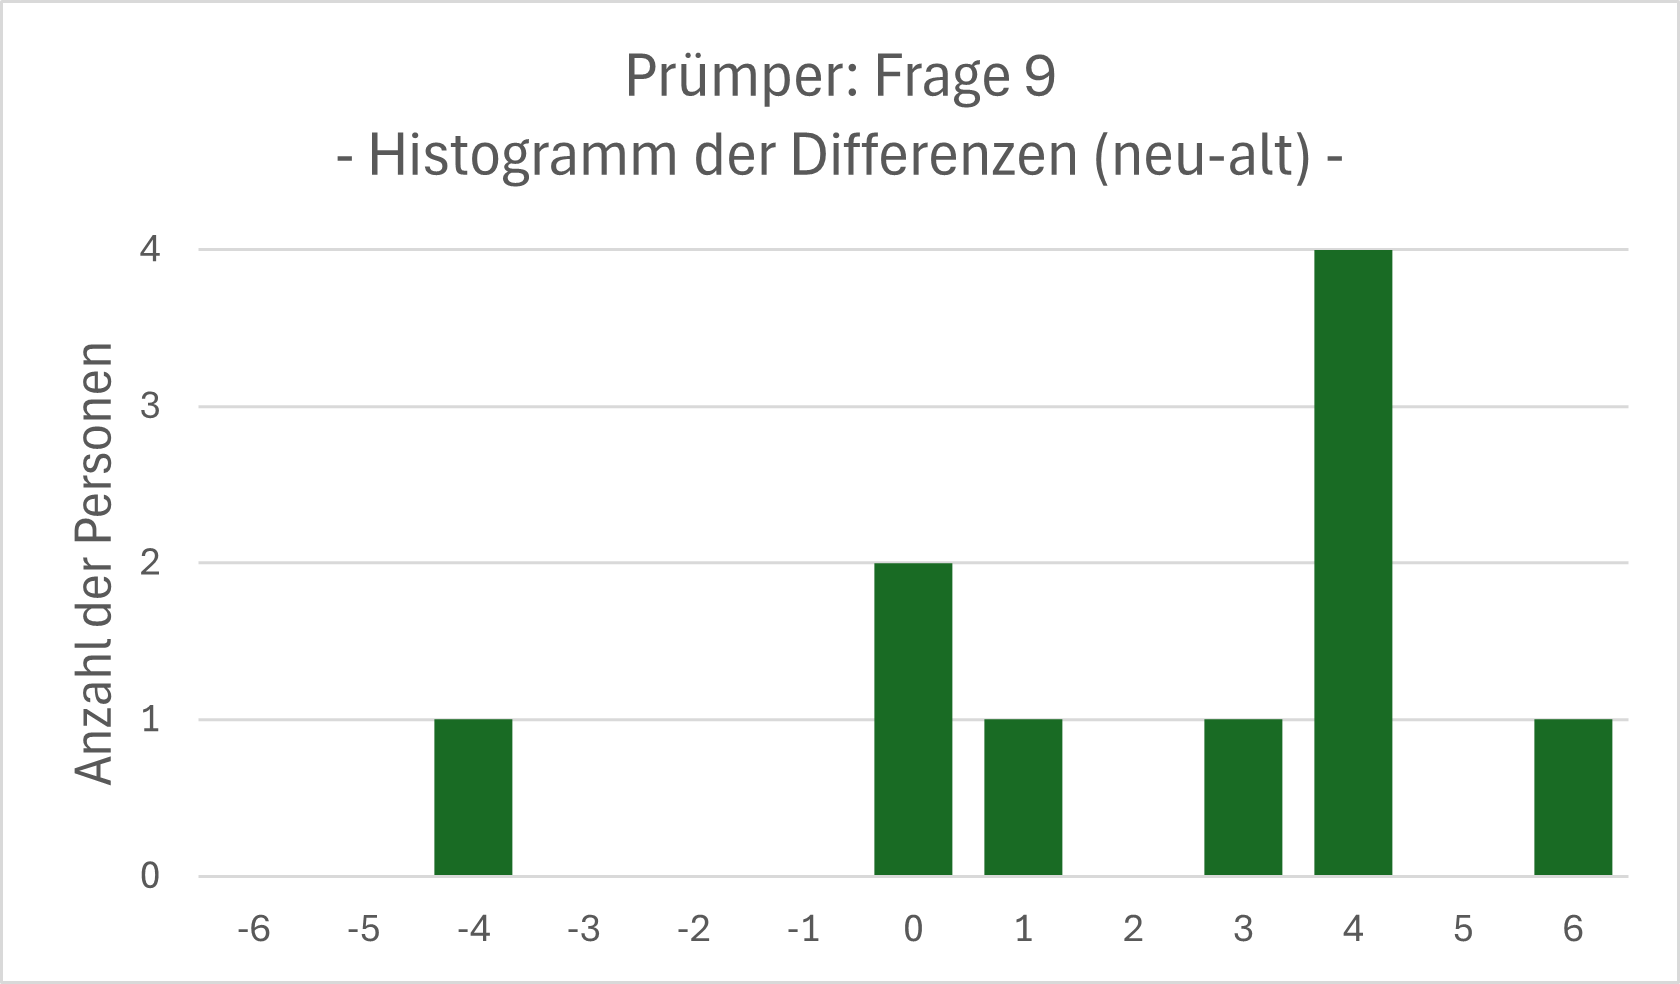
\includegraphics[width=0.45\linewidth]{Diagramme/hist_9_pruemper.png}
    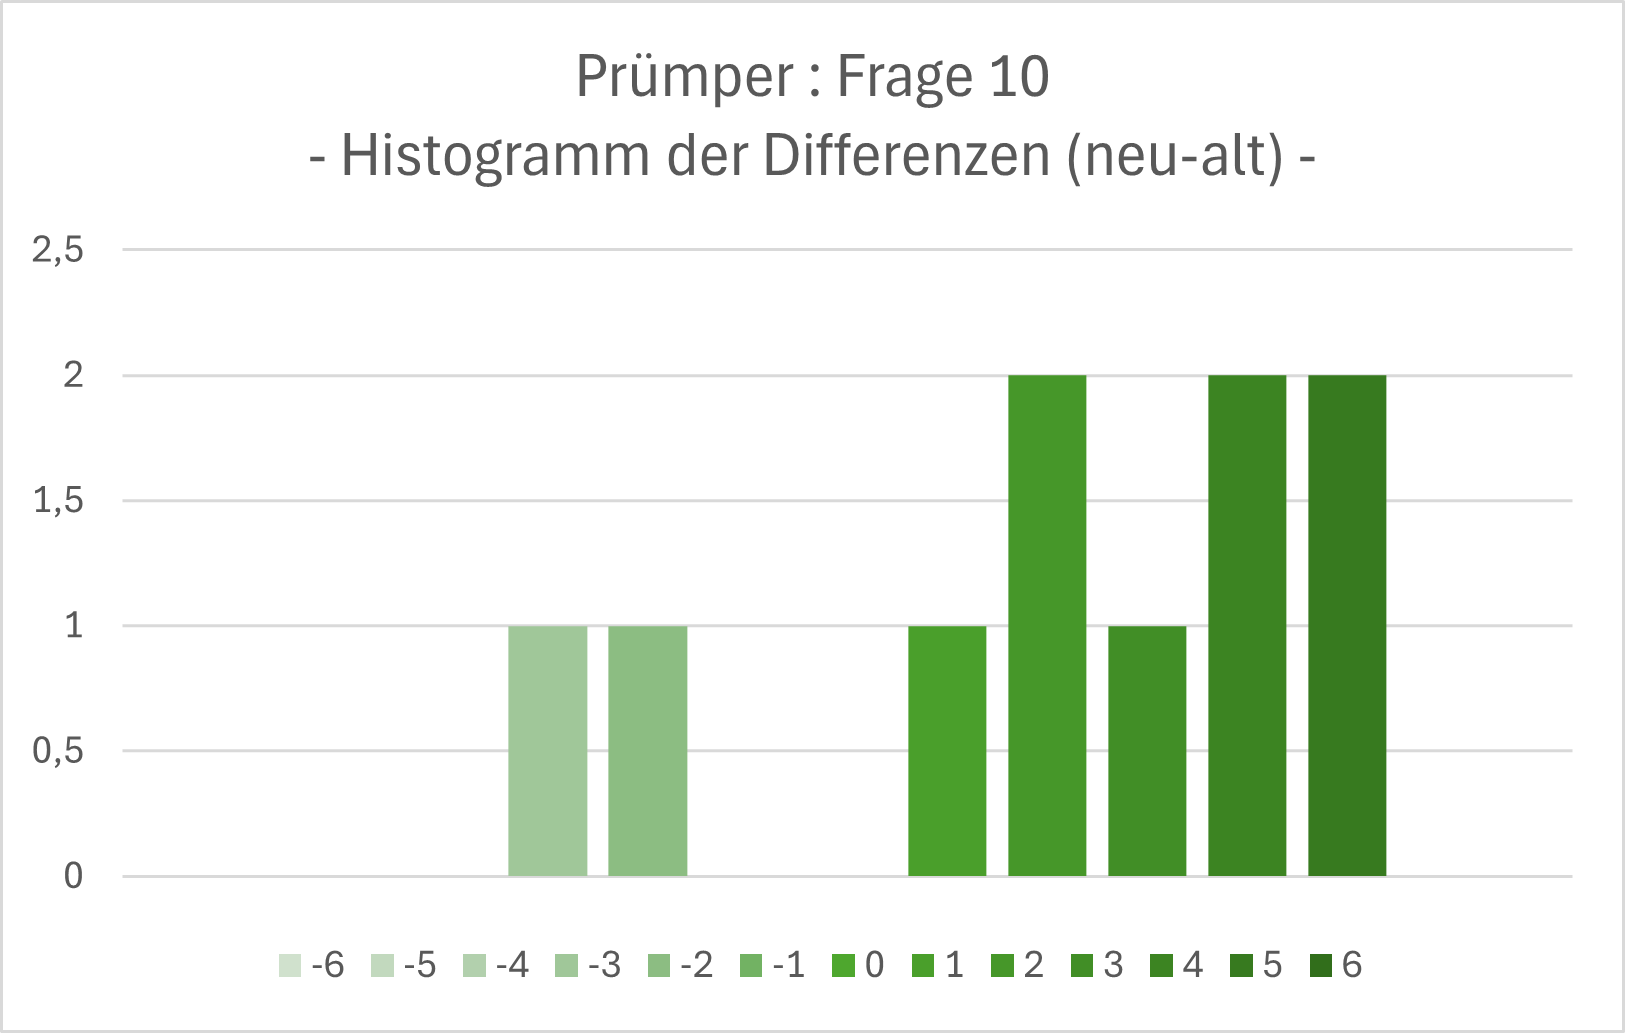
\includegraphics[width=0.45\linewidth]{Diagramme/hist_10_pruemper.png}

    \caption{Histogramme mit den Differenzen neu-alt der Nutzerbefragung}
    \label{fig:hist_prümper_all}
\end{figure}
\newpage

\section{\textcolor{Plum}{Ergebnisse nach Entfernung der Extrema aus Frage 2 und Frage 3}}
\label{Add:Pruemper:neuer_ttest:frage_2_und_3}

\textcolor{red}{TODO: auch die Ergebnisse je Reihenfolge einbeziehen}
-> rohe Daten ohne die Werte auflisten
--> welche Tabelle will ich? - die große mit allen oder nur die der beiden Fragen?
-> Grafik mit dem grünen Signifikanzniveau einbinden

\begin{table}[H]
    \centering
    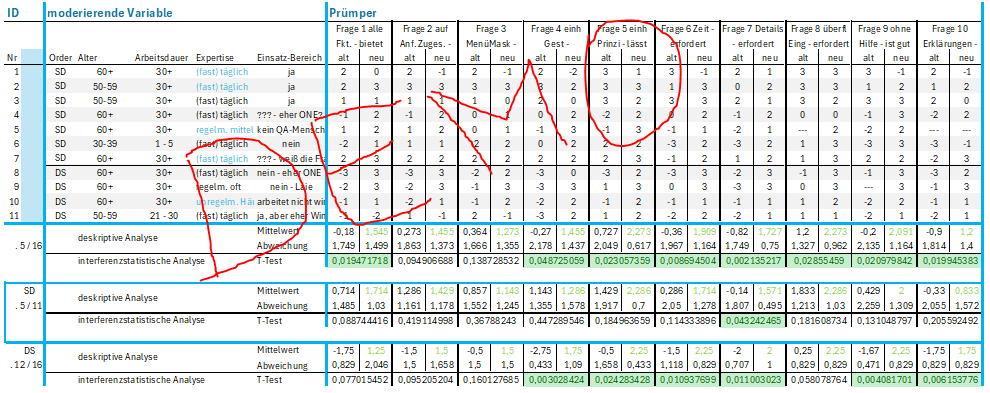
\includegraphics[width=0.65\textheight, angle=90]{Anhänge/Nutzerbefragung/prümper-Tabelle_demo.PNG}
    \caption{Nutzerbefragung nach Prümper der Fragen 2 und 3 nach Entfernung der Extrema - Tabellarische Daten \textcolor{red}{TODO: Bild austauschen}}
    \label{tab:Nutzerbefragung:rohe_Daten:ohne_Extrema_2_und_3}
\end{table}

\begin{figure}[H]
    \centering
    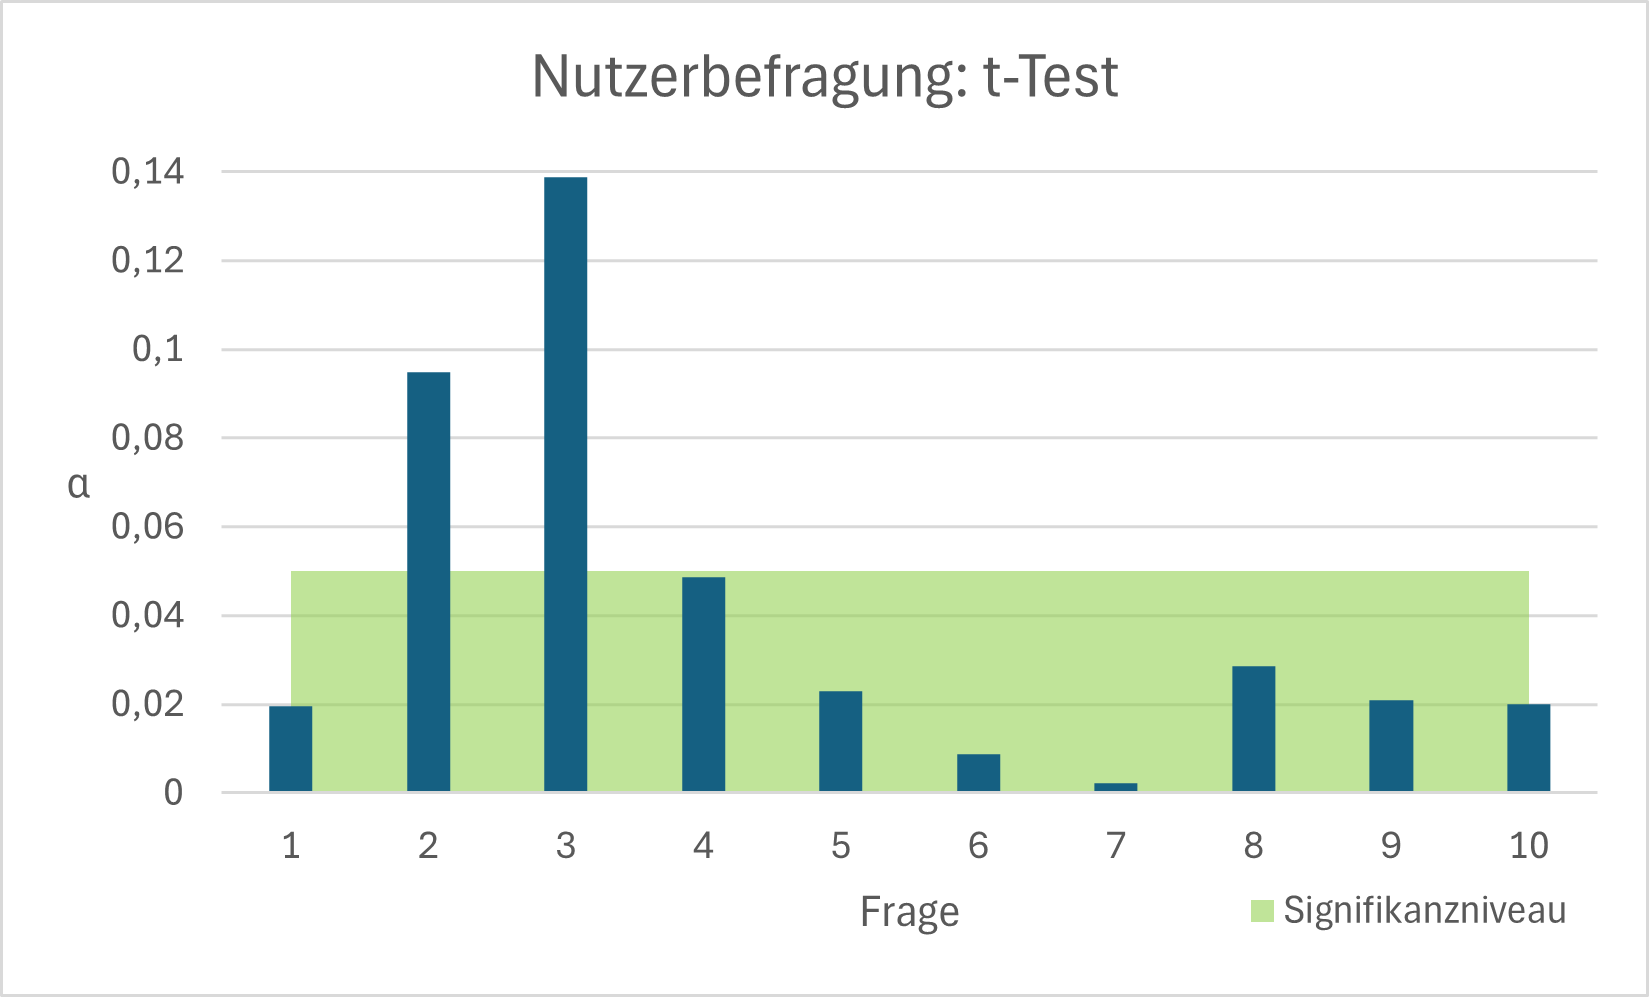
\includegraphics[width=0.8\linewidth]{Diagramme/pruemper_ttest.png}
    \caption{Nutzerbefragung - t-Test-Ergebnisse (Daten aus \autoref{tab:Nutzerbefragung:Differenz+ttest}) \textcolor{red}{TODO: neues Bild einfügen}}
    \label{fig:Nutzerbefragung:ttest+Signifikanzniveau:ohne_Extrema_2_und_3}
\end{figure}
\chapter{Anhänge zum Usability-Test}
\label{Add:Test}

- Aufgaben + Beschreibung \autoref{Add:Usability_Test:Aufgabenkatalog}\\
- Datentabelle %\label{fig:Usability_Test:rohe_Daten}\\
- Excel-Tabelle und Funktionen/Formeln \label{fig:Usability-Test:Excel_Berechnungen} \\
-> TTest \\
-> Fehlerquote \\
-> ...\\
- weitere nützliche Diagramme für die Auswertung\\

\section{Aufgabenkatalog}
\label{Add:Usability_Test:Aufgabenkatalog}

\noindent
\underline{Verwendete Fragen:} \textcolor{red}{TODO!}
\begin{itemize}
    \item Aufgabe 1: 
    \item Aufgabe 2: 
    \item Aufgabe 3.1: 
    \item Aufgabe 3.2: 
    \item Aufgabe 4.1: 
    \item Aufgabe 4.2: 
\end{itemize}

\noindent
\underline{Begründungen:} \textcolor{red}{TODO: unvollständig}\\
\label{Add:Usability_Test:Begündung_Aufgaben}

\begin{itemize}
    \item alle erwarteten Daten können durch eine klare Zahl im neuen System abgelesen werden
    \item es muss im neuen System nicht gezählt oder zusammengerechnet werden
    \item die Farbgestaltung im neuen System ist einheitlich gewählt
    \item es wurden verschiedene nicht-einheitliche Methoden der Informationsdarstellung abgefragt
\end{itemize}

\noindent
$\Rightarrow$ Alle oben genannten Gründe sind der angenommene Idealzustand. Ob das erfolgreich umgesetzt wurde zeigen die Ergebnisse (s. \autoref{ch:Ergebnisse})\\

\noindent
Aufgabe 1
\begin{itemize}
    \item ein einfacher Wert zum Ablesen
    \item Start einer Diskussion, da die Aufgabe mögliche 2 Lösungen hat
\end{itemize}

\noindent
Aufgabe 2
\begin{itemize}
    \item Abfrage eines weiteren Werts
    \item Addition von klaren Zahlen im alten System
\end{itemize}

\noindent
Aufgabe 3.1
\begin{itemize}
    \item Wechsel der allgemeinen Oberfläche, um zu testen ob die neue Ansicht mit dem 2. Dashboard intuitiv verstanden wird
    \item alte Oberfläche erfordert das Zusammenzählen von 'Err' oder 'OK'\\
    -> keine Zahlenangabe, wie viele Tests gut / nicht gut gelaufen sind
\end{itemize}

\noindent
Aufgabe 3.2
\begin{itemize}
    \item Aufmerksam machen, wie man auf das gleiche Ergebnis für das andere System gelangt
\end{itemize}

\noindent
Aufgabe 4.1
\begin{itemize}
    \item Wechsel der allgemeinen Oberfläche zurück zur ersten verwendeten Oberfläche
\end{itemize}

\noindent
Aufgabe 3.2
\begin{itemize}
    \item Aufmerksam machen, wie man auf das gleiche Ergebnis für das andere System gelangt
\end{itemize}

\newpage
\section{Vollständige und rohe Ergebnisse des Usability Test}

\begin{figure}[H]
    \centering
    \includegraphics[width=1\linewidth]{}
    \caption{\textcolor{red}{TODO: snippet von der Excel-Tabelle + Formel}}
    \label{fig:Usability_Test:rohe_Daten}
\end{figure}

% *********************************************************************************

\begin{table}[H]
\justifying
\begin{tabular}{|l|c|c|c|c|}
\hline
Aufgabe 1\textcolor{white}{.0}   & $\Bar{x}$ & $\Tilde{x}$ & $\sigma$ & f \\ \hline
alt                              & 16        &  13         &  11      &  0\%   \\ \hline
neu                              & 9,5       &  9          &  3,6     &  9,09\%   \\ \hline
%Differenz   &           &             & -     &  xxx   \\ \hline
%\end{tabular}
%\begin{tabular}{|l|c|c|c|c|}
\hline
Aufgabe 2\textcolor{white}{.0}   & $\Bar{x}$ & $\Tilde{x}$ & $\sigma$ & f \\ \hline
alt                              & 14        &  10         &  9,1  &  0\%   \\ \hline
neu                              & 6,5       &  6,5        &  2,3  &  30\%   \\ \hline
%Differenz   &           &             & -     &  xxx   \\ \hline
%\end{tabular}
%\begin{tabular}{|l|c|c|c|c|}
\hline
Aufgabe 3.1   & $\Bar{x}$ & $\Tilde{x}$ & $\sigma$ & f \\ \hline
alt           & 16        &  15         &  6,2  &  0\%   \\ \hline
neu           & 12        &  11         &  6,4  &  36,36\%   \\ \hline
%Differenz   &           &             & -     &  xxx   \\ \hline
\end{tabular}
\begin{tabular}{|l|c|c|c|c|}
\hline
Aufgabe 3.2   & $\Bar{x}$ & $\Tilde{x}$ & $\sigma$ & f \\ \hline
alt           & 9         &  8          &  5,4  &  0\%   \\ \hline
neu           & 5,4       &  4          &  3    &  36,36\%   \\ \hline
%Differenz   &           &             & -     &  xxx   \\ \hline
%\end{tabular}
%\begin{tabular}{|l|c|c|c|c|}
\hline
Aufgabe 4.1   & $\Bar{x}$ & $\Tilde{x}$ & $\sigma$ & f \\ \hline
alt           & 21        &  18         &  7,4  &  45,45\%   \\ \hline
neu           & 15        &  12         &  8,8  &  9,09\%   \\ \hline
%Differenz   &           &             & -     &  xxx   \\ \hline
%\end{tabular}
%\begin{tabular}{|l|c|c|c|c|}
\hline
Aufgabe 4.2   & $\Bar{x}$ & $\Tilde{x}$ & $\sigma$ & f \\ \hline
alt           & 12        &  11         &  7,7  &  18,18\%   \\ \hline
neu           & 8,5       &  7          &  4,4  &  9,09\%   \\ \hline
%Differenz   &           &             & -     &  xxx   \\ \hline
\end{tabular}

\begin{tabular}{ll}
\multicolumn{2}{l}{verwendete Formelzeichen:} \\ \hline
$\Bar{x}$          & Mittelwert               \\
$\Tilde{x}$        & Median                   \\
$\sigma$           & Standardabweichung       \\
f                  & Fehlerquote
\end{tabular}
\caption{Zusammenfassung der Ergebnisse des Usability-Tests (Weiterverarbeitung der Daten aus \autoref{fig:Usability_Test:rohe_Daten})}
\label{tab:usability_test:mittelwerte}
\end{table}

% *********************************************************************************

\begin{table}[H]
\begin{tabular}{|l|c|c|c|c|c|c|}
\hline
                                          & Frage 1 & Frage 2 & Frage 3.1 & Frage 3.2 & Frage 4.1 & Frage 4.2 \\ \hline
$\varnothing t_{neu} - \varnothing t_{alt}$ & -6,55   & -7,14   & -4,46     & -3,64     & -6,18     & -3,81     \\ \hline
T-Test                                    & 0,0231  & 0,0186  & 0,0579    & 0,0506    & 0,0554    & 0,0826    \\ \hline
\end{tabular}
\caption{Usability Test - Differenz der Zeitmittelwerte und T-Test-Ergebnisse (Weiterverarbeitung der Daten aus \autoref{tab:usability_test:mittelwerte} und \autoref{fig:Usability_Test:rohe_Daten})}
\label{tab:usability_test:Differenz+ttest}
\end{table}

\textcolor{red}{TODO: weitere T-Tests von Aufgaben 2+3}\\
?? hier? oder war ddas bei der Nutzerbefragung?

%*************************************************************************
% Other Stuff in the Back
%*************************************************************************
\cleardoublepage%********************************************************************
% Bibliography
%*******************************************************
% work-around to have small caps also here in the headline
% https://tex.stackexchange.com/questions/188126/wrong-header-in-bibliography-classicthesis
% Thanks to Enrico Gregorio
\defbibheading{bibintoc}[\bibname]{%
  \phantomsection
  \manualmark
  \markboth{\spacedlowsmallcaps{#1}}{\spacedlowsmallcaps{#1}}%
  \addtocontents{toc}{\protect\vspace{\beforebibskip}}%
  \addcontentsline{toc}{chapter}{\tocEntry{#1}}%
  \chapter*{#1}%
}

% allow Linebreaks in urls anywhere
\setcounter{biburlnumpenalty}{100}
\setcounter{biburlucpenalty}{100}
\setcounter{biburllcpenalty}{100}
% enable to long words to break anywhere by increasing the allowed whitespace between words.
\sloppy

\printbibliography[heading=bibintoc]


%*************************************************************************
% Game Over: Restore, Restart, or Quit?
%*************************************************************************
\end{document}
%*************************************************************************
